\documentclass{article}


% Language setting
% Replace `english' with e.g. `spanish' to change the document language
% \usepackage[english]{babel}

% Set page size and margins
% Replace `letterpaper' with `a4paper' for UK/EU standard size
%\usepackage[letterpaper,top=2cm,bottom=2cm,left=3cm,right=3cm,marginparwidth=1.75cm]{geometry}

% Useful packages
\usepackage{amsmath}
\usepackage{tikz}
\usetikzlibrary{trees}
\usetikzlibrary{positioning} 
\usetikzlibrary{arrows}
\usetikzlibrary{decorations.pathmorphing}
\usetikzlibrary{shapes.multipart}
\usetikzlibrary{shapes.geometric}
\usetikzlibrary{calc}
\usetikzlibrary{positioning} 
\usetikzlibrary{fit}
\usetikzlibrary{backgrounds}
\usetikzlibrary{automata}
\usepgflibrary{shapes.geometric}
\usetikzlibrary{shapes.geometric}
\usepackage{mathpartir}
\usepackage{listings}
\usepackage{proof}
\newtheorem{theorem}{Theorem}
\newtheorem{lemma}{Lemma}

\usepackage{graphicx}
%\usepackage[colorlinks=true, allcolors=blue]{hyperref}


\lstdefinelanguage{L4}
{morekeywords={
      assert 
    , class  
    , decl   
    , defn   
    , extends
    , lexicon
    , fact   
    , rule   
    , derivable
    , let   
    , in    
    , not   
    , forall
    , exists
    , if   
    , then 
    , else 
    , for  
    , true 
    , false
},    
sensitive=false,
morecomment=[l]{\#},
morestring=[b]",
}

\lstset{frame=tb,
  language=L4,
  aboveskip=3mm,
  belowskip=3mm,
  showstringspaces=false,
  columns=flexible,
  basicstyle={\footnotesize\ttfamily},
  numbers=none,
  numberstyle=\tiny\color{gray},
  keywordstyle=\color{blue},
  commentstyle=\color{green},
  stringstyle=\color{mauve},
  breaklines=true,
  breakatwhitespace=true,
  tabsize=2
}

%%% Local Variables: 
%%% mode: latex
%%% TeX-master: "main"
%%% End: 





\title{User Guided Abductive Proof Generation for Answer Set Programming Queries}
\author{You}

\begin{document}
\maketitle

\begin{abstract}
 We present a method for generating possible proofs of a query with respect to a given Answer Set Programming (ASP) rule set using an abductive process where the space of abducibles is automatically constructed just from the input rules alone. Given a (possibly empty) set of user provided facts, our method infers any additional facts that may be needed for the entailment of a query and then outputs these extra facts, without the user needing to explicitly specify the space of all abducibles. We also present a method to generate a set of directed edges corresponding to the the justification graph for the query. Furthermore, through different forms of implicit term substitution, our method can take user provided facts into account and suitably modify the abductive solutions. Past work on abduction has been primarily based on goal directed methods. However these methods can result in solvers that are not truly declarative. Much less work has been done on realizing abduction in a bottom up solver like the Clingo ASP solver. We describe novel ASP programs which can be run directly in Clingo to yield the abductive solutions and directed edge sets without needing to modify the underlying solving engine. 
\end{abstract}

\section{Introduction}
The goal of this paper is to describe a method to automatically genenrate a space of abducibles, that will allow the creation of a fact set that results in the entailment of a given query with respect to a given ASP rule set. \\
\newline
A novel feature of the method is that depth control for proof search is done in a purely declarative way as part of the proof search encoding itself. Furthermore, adding facts to the program automatically triggers a kind of controlled variable substitution where skolem terms or other 'place-holder' terms occurring in abducibles are replaced away so that the resulting proof is simplified, without any need for an explicit representation of equality between terms. We present two main sets of proof-search encodings. One is guaranteed to only produce finite answer sets, but which does not support complete variable substitution in abducibles. The other encoding may produce infinite answer sets in the presence of skolem functions but supports complete variable substitution and still only produces finite answer sets if there are no skolem terms involved. Next we present an encoding which generates a set of directed edges representing a justification graph of any desired depth. The novel encodings for variable substitution and depth control set this work apart from other attempts like [Schuller ref, Petr Homola ref] to realize abduction in a Clingo-like bottom-up reasoner. Unlike sCASP our method keeps the justification production and proof search separate from each other which allows the user to have greater control on the justification produced without affecting the proof search procedure. Furthermore, in general, abduction problems where the input rules involve function symbols often either lead to infinite grounding or infinite backward proof search and problems that are intractable with a top-down reasoning mechanism often yield to a bottom-up reasoner and vice versa. Lastly, as mentioned in the abstract, there may be use cases where one wants to know all the resulting consequences of an abductive solution to a query with respect to a rule-set. Informally one can relate this to the problem of \emph{bi-abduction} which has been explored in separation logic [Bi-ab ref]. Hence our work can be regarded as addressing the problem of \emph{bi-abduction} but in an ASP setting. (However we shall not dwell on this connection any further, instead focus only on the abductive reasoning process). Therefore an abductive reasoner based on a solver like Clingo can complement the abilities of goal directed reasoners like sCASP, CIFF etc.  The rest of the paper is organised as follows. Section~\ref{sec:abductive_proof} provides some further background and motivation for the subject of the paper and also describes the problem being tackled more formally. Section~\ref{sec:derived_asp} presents 3 core sets of meta-rules that facilitate the abductive proof generation process. Section~\ref{sec:sample_problem} describes some formal results about the generated proof trees. Section~\ref{sec:proof_finiteness} discusses applications and comparisons to other work and Section~\ref{sec:conclusion} concludes. 

\paragraph{Example of proof tree}

$
\infer[(E\wedge_1)]{\Gamma \vdash A}{
  \infer{\Gamma \vdash A \wedge B}{\vdash A & \vdash B}
  }
\qquad
\infer[(E\wedge)]{\Gamma \vdash B}{\Gamma \vdash A \wedge B}
$ 

\paragraph{Example using Tikz}

\begin{figure}[h]
\begin{center}
  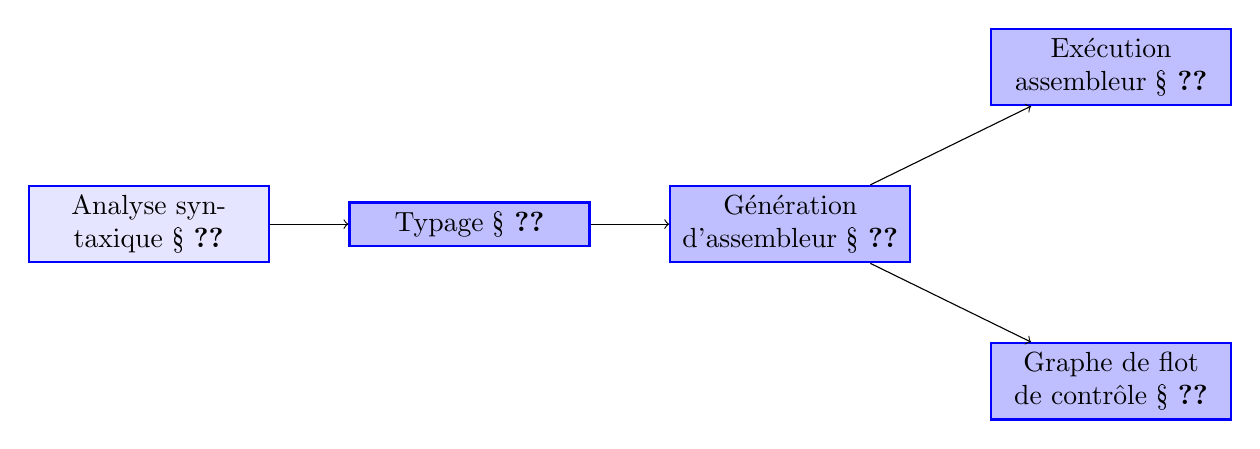
\begin{tikzpicture}[
auto,
light/.style ={rectangle, draw=blue, thick, fill=blue!10,
  text width=8em, text centered, 
  minimum height=1em
},
dark/.style ={rectangle, draw=blue, thick, fill=blue!25,
  text width=8em, text centered, 
  minimum height=1em},
line/.style ={draw, -latex'},
dotline/.style ={draw, dotted, -latex'},
thickline/.style ={draw, thick, -latex'}
]

\node[light] (ans) {Analyse syntaxique \S~\ref{sec:ans}};
\node[dark] (typ) [right=of ans] {Typage \S~\ref{sec:typ}};
\node[dark] (gen) [right=of typ] {Génération d'assembleur \S~\ref{sec:gen}};
\node[dark] (exec) [above right=of gen] {Exécution assembleur \S~\ref{sec:exec}};
\node[dark] (graph) [below right=of gen] {Graphe de flot de contrôle \S~\ref{sec:graph}};

\path[->]
(ans) edge (typ)
(typ) edge (gen)
(gen) edge (exec)
(gen) edge (graph)
;
\end{tikzpicture}
\end{center}
\caption{Tikz example}
\end{figure}


\begin{figure}

    \begin{center}
  \begin{tikzpicture}
  [level distance = 8mm,
  level 1/.style={sibling distance=30mm},
  level 2/.style={sibling distance=20mm},
  level 3/.style={sibling distance=10mm},
  level 4/.style={sibling distance=18mm},
  level 5/.style={sibling distance=8mm},
  ]

  \node {$\vee$}
  child {node {$\wedge$}
    child {node {p}
    }
    child {node {q}
    }
  }
  child {node {$\lnot$}
    child {node {$\vedge$}
      child {node {p}
      }
      child {node {r}
      }
    }
  };
  \end{tikzpicture}
\end{center}

\caption{Trees}
\end{figure}

\section{Abductive Proof Generation Task}\label{sec:abductive_proof}
\subsection{Formal Setup}
Given a source ASP rule set $R$, let the tuple $<R,q,U,C,N>$ denote the tuple consisting of the source ASP rules $R$, a ground positive or negative atom $q$. The set $U$ consists of 2 subsets. First we have a set of user-inputed facts, where each fact $f$ is denoted by the atom $user\_input(pos,f)$. Next in $U$ we have set of integrity constraints that constrain which atoms may be abduced. For example the constraint $:-abducedFact(p(X)).$ means no instantiation of the predicate $p$ maybe abduced.The integrity constraints can also prevent only specific instances of predicates from being abduced. For example instead of the constraint above we may have the constraint $:-abducedFact(p(john)).$.  $C$ denotes a set of ASP constraint which constrain which atoms may or may not appear in the complete model that results from the rules and abducibles. Finally we have the non-negative integer $N$. This acts as the depth control parameter for abductive proof search. We shall exemplify all these definitions with some examples later on. Then the key task is to find a set of facts $F$, such that:

\begin{enumerate}
    \item If $q$ is a positive atom, it is in some answer set $\mathcal{A}$ of $F\cup R\cup C$. If $q$ is a NAF atom, then there exists an answer set $\mathcal{A}$ of $F\cup R\cup C$ such that $q$ is $not$ in $\mathcal{A}$.
    \item $F$ contains all the positive facts from $U$ and $F$ does not violate any of the integrity constraints in $U$ Ie. $F$ does not contain abducibles that are specifically disallowed by the constraints on abducibles in $U$.
    \item $F$ does not have any atoms whose depth level is greater than $N$.
\end{enumerate}
We say $F$ is a solution of the abductive proof generation task $<R,Q,U,C,N>$

\subsection{Source ASP program}

When considering any abductive proof generation task we make the following assumptions on the input ASP rule set $R$. We assume that each source ASP rule has exactly the following form:
\begin{verbatim}
pre_con_1(V1),pre_con_2(V2),...,pre_con(Vk),not pre_con(Vk+1),...,not pre_con_n(Vn) -> post_con(V).
\end{verbatim}
We further make the folllowing assumptions:

\begin{enumerate}
    \item Each pre-condition $pre\_con_{i}(V_{i})$ is atomic and so is the post-condition $post\_con(V)$.
    \item The $not$ in front of the pre-conditions denotes \textit{negation as failure} interpreted under the \textit{stable model semantics}
    \item $V_{i}$ is the set of variables occuring in the $i^{th}$ pre-condition which is either $pre\_con_{i}(V_{i})$ or $not$ $pre\_con_{i}(V_{i})$ and $V$ is the set of variables occuring in the post condition $post\_con(V)$. We assume that $V\subseteq V_{1}\cup V_{2}\cup ... \cup V_{n}$.
    \item Each variable occurring in the post condition is universally quantified over, and each variable that occurs in some pre-condition but not the post condition is existentially quantified. In particular together with (3), this means that there are no existentially quantified variables in rule post-conditions.
    \item Each variable that occurs in a negation-as-failure pre-condition also occurs in some positive pre-condition.
    \item Each input rule of the form above is assigned some unique rule.id.
\end{enumerate}

We further assume that given any integrity constraint $c$ in $C$, every variable in a negation-as-failure atom in $c$ also occurs in some positive atom in $c$. We will now define the depth level of an atom with respect to a given input source ASP rule set $R$ and query $q$.
\subsection{Depth level of an atom}
We define a map $\phi$ that maps an atom to a set of non-negative integers. We will describe this map rather informally. For the query $q$, $0\in \phi(q)$. Now the rest of the definition is recursive. Given an atom $a$, the non-negative integer $n$, $n\in \phi(a)$ if and only if there exists a rule $r$ in $R$ such that there is a substitution $\theta$ of the variables in $r$ such that there exists some precondition (negated or positive) $p$ of $r$ such that that $\theta$ applied to $p$ gives $a$ and $\theta$ applied to the post condition of $r$ gives some atom $a'$ where $n-1$ $\in$ $\phi(a')$. \\
\newline
Given an atom $a$ let $\phi_{min}(a)$ be $-1$ if the set $\phi(a)$ is empty and let $\phi_{min}(a)$ be the minimum member of the set $\phi(a)$ otherwise. Then $\phi_{min}(a)$ is defined to be the $depth$ $level$ of $a$ with respect to the rule set $R$ and query $q$.  

\section{Derived ASP Programs}\label{sec:derived_asp}
Before we give the details of the main sets of rule translations that allow abductive reasoning and justification generation, here is a simple example to illustrate some key ideas and what the desired output for an abductive problem is. Consider the rule set $R$ given by the 3 rules
\begin{verbatim}
1) p(X,Y):-q(X,Y),r(X),s(Y).
2) p(X,Y):-g(X,Y).
3) d(X,Y):-g(X,Y).
\end{verbatim}
Now let $q$ be $p(john,james)$, let $U$ consist of the user provided fact $r(john)$ and let $U$ also include the constraint on abducibles $:-p(X,Y)$ meaning that no instance of the predicate $p$ may be abduced. Next let the set $C$ contain the single constraint $:-d(X,Y)$ meaning that we require a stable model of the user given facts, the abducibles, and the rules, which does not contain any instance of the predicate $d$, finally let $N = 2$. Then for this problem the minimal abductive solution can be represented by $\textit{abducedFact(q(john,james)), abducedFact(s(james))}$, which is what we want to get out of our encoding. Intuitively, the way we will solve this abductive reasoning problem is by first encoding the input rules such as the ones above directly as they are. Then we will have a representation which corresponds to 'reversing' the rules, ie we go from post-conditions to pre-conditions. These 'reveresed' rules generate a maximal space of abducibles which then feed into the direct rule translation. Finally we will have integrity constraints that ensure that the atom which we want to be true (represented by $q$) is indeed entailed by the abductive solution. An adapted version of this 'reversed rule' representation also enables us to generate a set of directed edges corresponding to a justification graph. The technical challenge in this process comes from finding a way to control the depth of abduction space generation. The other key challenge is dealing with rules that may have existential variables in pre-conditions or when rules may not have existential quantifier but the goal represented by $q$ is un-ground or existential in nature. So for example it maybe the case that the goal is not $p(john,james)$ but any arbitrary instance of the predicate $p$.    

\subsection{Core rule translations}

\subsubsection{Core Forward Reasoning}
Given an input rule \begin{verbatim}
pre_con_1(V1),pre_con_2(V2),...,pre_con(Vk),not pre_con(Vk+1),...,not pre_con_n(Vn) -> post_con(V).
\end{verbatim} obeying all the properties as above we write the following rule in our ASP program: 
\begin{verbatim}
holds(post_con(V)):-holds(pre_con(V1)),...,holds(pre_con(Vk)), not holds(pre_con(Vk+1)),...
,not holds(pre_con(Vn)). 
\end{verbatim}   
We repeat this for each source ASP rule. For each constraint in $C$, we simply enclose each atom in the constraint inside the $holds$ predicate. For example if $C$ contains the constraint $:-b(X,Y).$, (meaning that we require an abductive solution such that the there exists a stable model of the abduced facts, rules and user provided facts, which contains no instantiations of the predicate $b$), we encode that constraint as:
\begin{verbatim}
:-holds(b(X,Y)).
\end{verbatim}
\subsubsection{Generating Abducibles}
For this next set of meta-rules we will first need a way to assign the appropriate skolem terms to existential variables in pre-conditions. First given some rule in our rule set, say rule $r_{j}$. We now fix some order $O_{r_{j}}$ on the variables occuring in the combined set of variables from the post and pre-conditions of the rule $r_{j}$. Now we will describe a skolemnization map that assigns an existential variable in a pre-condition of $r_{j}$ to a skolem term. Firstly, let the rule $r_{j}$ 
carry unique integer id. $t$. Let $v$ be a variable that occurs in some rule precondition but not the post condition. Then under this skolemization map, the variable $v$ gets mapped to \begin{verbatim}
skolemFn_t_v_(V)    
\end{verbatim}
where $V$ denotes the variables in the post-condition occuring in the order inherited from $O_{r_{j}}$. For example consider the rule $r$: \begin{verbatim}
p(Y,X):- q(X),r(X,Y),s(Z).    
\end{verbatim} 
Assume that this rule carries integer id $1$. Let $O_{r}$ be $[X,Y,Z]$. Then the variable $Z$ gets mapped to the skolem term $skolemFn\_1\_Z(X,Y)$.\\
\newline
\subsubsection{AG1}
Given an input ASP rule $r$ in $R$
\begin{verbatim}
pre_con_1(V1),pre_con_2(V2),...,pre_con(Vk),not pre_con(Vk+1),...,not pre_con_n(Vn) -> post_con(V).
\end{verbatim}
our first set of abducible generation/proof search rules $AG1$ is given by the following. (In the rest of the paper we will use the terms abducible generation rules and proof search rules interchangeably) 
\begin{verbatim}
create_subs(sub_Inst_t((V'_sk),N+1):-query(post_con(V),N),N<M-1.
\end{verbatim}
Here $V'_{sk}$, denotes the ordered list $O_{r}$ but with existential variables replaced by their skolem term counter parts. Here $t$ is the integer id for the rule.
Next we have the following rules:
\begin{verbatim}
explains(pre_con_1(V1),post_con(V),N):-create_subs(sub_Inst_t((V'),N).
explains(pre_con_2(V2),post_con(V),N):-create_subs(sub_Inst_t((V'),N).
                          .
                          .
                          .
                        
explains(pre_con_n(Vn),post_con(V),N):-create_subs(sub_Inst_t((V'),N).
\end{verbatim}
Here $V'$ denotes the ordered list $O_{r}$. \\
\newline
\subsubsection{AG2}
Now we shall construct the second set of proof search rules $AG2$ Given $O_{r}$ construct $F_{r}$ be adjoining $FreshVar$ to each entry of $O_{r}$. So for our example above $F_{r}$ becomes $[FreshVar\_X,FreshVar\_Y,FreshVar\_Z]$. Given a pre condition $p$ occurring in $r$ $M_{r,p}$ is an ordered list constructed as follows. The $i_{th}$ element of $M_{r,p}$ is the $i_{th}$ element of $O_{r}$ if the $i_{th}$ element of $O_{r}$ is a variable which occurs in $p$. Otherwise, the $i_{th}$ element of $M_{r,p}$ is given by the $i_{th}$ element of $F_{r}$. Now for each negated or positive precondition $p$ we have the following rule:
\begin{verbatim}
 create_subs(sub_Inst_t(M_(r,p)),M-1):-create_subs(sub_Inst_t(F_r),N),holds(p),max_ab_lvl(M), N<M.   
\end{verbatim}
Repeat this for each pre-condition and. This is the set of rules $AG2$. \\
\newline
\subsubsection{AG3}
Finally $AG3$ consists of just the single rule:
\begin{verbatim}
query(X,N):-explains(X,Y,N),max_ab_lvl(M),N<M.
\end{verbatim}
\subsubsection{Skolem Example}
Let us consider another example

Consider the source ASP rule:
\begin{verbatim}
a(X):- b(X,Y,Z), not c(X), not d(Y) .    
\end{verbatim}
Say this rule $r$ has rule id. $5$. 
Let $O_{r}$ be $[X,Y,Z]$ Here is the encoding for the rule, $AG1$ is:
\begin{verbatim}
create_subs(subs_Inst_5(X,skolemFn_5_Y(X),skolemFn_5_Z(X),N+1):-query(a(X),N),max_ab_lvl(M),N<M-1.


explains(b(X,Y,Z),a(X),N):-create_subs(subs_Inst_5(X,Y,Z),N).

explains(c(X),a(X),N):-create_subs(subs_Inst_5(X,Y,Z),N).

explains(d(Y),a(X),N):-create_subs(subs_Inst_5(X,Y,Z),N).

\end{verbatim}
AG2 is given by:
\begin{verbatim}
create_subs(subs_Inst_5(X,Y,Z),M-1):-create_subs(subs_Inst_5(FreshVar_X,FreshVar_Y,FreshVar_Z),N), 
holds(b(X,Y,Z)),max_ab_lvl(M),N<M.

create_subs(subs_Inst_5(X,FreshVar_Y,FreshVar_Z),M-1):-
create_subs(subs_Inst_5(FreshVar_X,FreshVar_Y,FreshVar_Z),N), holds(c(X)),max_ab_lvl(M),N<M.

create_subs(subs_Inst_5(FreshVar_X,Y,FreshVar_Z),M-1):-
create_subs(subs_Inst_5(FreshVar_X,FreshVar_Y,FreshVar_Z),N), holds(d(Y)),max_ab_lvl(M),N<M.
\end{verbatim}
\subsubsection{Supporting code for Abduction} 
Given the original problem $<R,q,U,C,N>$, set $M=N+1$. Then we have the following: 
\begin{verbatim}
max_ab_lvl(M).
query(Q,0):-generate_proof(Q).
{abducedFact(X)}:-query(X,M).
holds(X):-abducedFact(X).

holds(X):-user_input(pos,X).
\end{verbatim}
For any predicate $p$, say of arity $n$ such that no instance of $p$ may be abduced, we add the constraint.
\begin{verbatim} 
:-abducedFact(p(X1,X2,...,Xn).
\end{verbatim}
If instead only a specific ground instance of $p$ or a partially ground instance of $p$ should be prevented from being abduced then we simply adapt the above constraint accordingly. For instance if $p$ is a binary predicate and we want that no instance of $p$ where the first argument is $alpha$ should be adbuced we have the constraint
\begin{verbatim} 
:-abducedFact(p(alpha,X)).
\end{verbatim}
Next we add the following $weak$ constraint so that in the optimal abductive solution as few abducibles as possible are used.
\begin{verbatim} 
:~abducedFact(X).[1@1,X]
\end{verbatim}
\subsubsection{Specifying the goal}
Here is the code to encode the goal of the abductive reasoning process. If our goal is ground atom say $p(a1,a2..,an)$ for some predicate $p$ then we have:
\begin{verbatim}
generate_proof(p(a1,a2,...,an)).
goal:-holds(p(a1,a2,..,an)).
:- not goal.
\end{verbatim}
If on the other hand our goal is unground or only partially ground then we have the following. Say our goal is of the form $p(a,X,b,Y,Y)$, which means that $X$,$Y$ are existential variables. Then for the example we have the following:
\begin{verbatim}
generate_proof(p(a,v1,b,v2,v2)).
goal:-holds(p(a,X,b,Y,Y)).
:- not goal.
\end{verbatim}
Here $v1$, $v2$ are fresh constants.

\subsection{Extending abduction generation space for rules without existential variables}
When we have rules without existential variables, we can construct a larger space of abducibles without worrying about our ASP programs having infinite answer sets because there are now no skolem expressions. The encoding $AG1$ is the same as before but now clearly there will be no skolem terms. The new version of $AG2$ which we shall call $AG2_{exp}$ now becomes for each rule
\begin{verbatim}
 create_subs(sub_Inst_t(M_(r,p)),N):-create_subs(sub_Inst_t(F_r),N),holds(p),max_ab_lvl(M), N<M.   
\end{verbatim}
Repeat this for each pre-condition $p$. Then for the post-condition of the rule $p'$, we have:
\begin{verbatim}
 create_subs(sub_Inst_t(M_(r,p')),N):-create_subs(sub_Inst_t(F_r),N),holds(p'),max_ab_lvl(M), N<M.   
\end{verbatim}
Here $M_{r,p'}$ is defined exactly the same way as $M_{r,p}$ for some pre-condition $p$. Next, for each rule and for each pre-condition $p$ in the rule we have.
\begin{verbatim}
 create_subs(sub_Inst_t(M_(r,p)),N):-create_subs(sub_Inst_t(F_r),N),query(p,N),max_ab_lvl(M), N<M.   
\end{verbatim}
For the post-condition $p'$ we have:
\begin{verbatim}
 create_subs(sub_Inst_t(M_(r,p')),N):-create_subs(sub_Inst_t(F_r),N),query(p',N-1),max_ab_lvl(M),0<N,N<M.   
\end{verbatim}
This completes the encoding $AG2_{exp}$. The adapted version of $AG3$ $AG3_{exp}$ is given by adding to $AG3$ one extra rule. So $AG3_{exp}$ is:
\begin{verbatim}
query(X,N):-explains(X,Y,N),max_ab_lvl(M),N<M.
query(Y,N-1):-explains(X,Y,N),max_ab_lvl(M),1<N,N<M.
\end{verbatim}
\subsection{Discussion of Abduction space generation}
\subsubsection{Full term substitution}
We first give an example of the expanded abduction space encoding to explain the intuition behind various parts of the encoding. Consider the rule set below that has no existential variables but which has negation as failure and where the goal is un-ground. 
\begin{verbatim}
relA(X,Y):-relB(X,Y), relD(Y), not relE(Y).
relE(Y):-relD(Y), not relF(Y).
\end{verbatim}
Let the goal $q$ be $relA(P,R)$, where $P$,$R$ are un-ground existential variables. Next suppose that the only constraint on abducibles is that no instantiation of $relA$ can be abduced and further suppose that the set of user provided facts is initially empty. Finally let $N=4$. Here is the complete encoding for this problem. 

\begin{lstlisting}[language=Prolog, numbers=left]
max_ab_lvl(5).
% Encoding the goal
generate_proof(relA(v1,v2)).
query(X,0):-generate_proof(X).
goal:-holds(relA(P,R)).
:- not goal.

% Core rule translation
holds(relA(X,Y)) :- holds(relB(X, Y)),holds(relD(Y)), not holds(relE(Y)).
holds(relE(Y)) :- holds(relD(Y)), not holds(relF(Y)).

% AG1_exp
createSub(subInst_r1(X,Y),N+1) :- query(relA(X,Y) ,N),max_ab_lvl(M),N<M-1.
createSub(subInst_r2(Y),N+1) :- query(relE(Y) ,N),max_ab_lvl(M),N<M-1.

explains(relB(X, Y), relA(X,Y) ,N) :- createSub(subInst_r1(X,Y),N).
explains(relD(Y), relA(X,Y) ,N) :- createSub(subInst_r1(X,Y),N).
explains(relE(Y), relA(X,Y) ,N) :- createSub(subInst_r1(X,Y),N).


explains(relD(Y), relE(Y) ,N) :- createSub(subInst_r2(Y),N).
explains(relF(Y), relE(Y) ,N) :- createSub(subInst_r2(Y),N).


% AG2_exp for rule 1

createSub(subInst_r1(X,Y),N) :- createSub(subInst_r1(V_X,V_Y),N), holds(relA(X,Y)).
createSub(subInst_r1(X,Y),N) :- createSub(subInst_r1(V_X,V_Y),N), holds(relB(X,Y)).
createSub(subInst_r1(V_X,Y),N) :- createSub(subInst_r1(V_X,V_Y),N), holds(relD(Y)).
createSub(subInst_r1(V_X,Y),N) :- createSub(subInst_r1(V_X,V_Y),N), holds(relE(Y)).

createSub(subInst_r1(X,Y),N) :- createSub(subInst_r1(V_X,V_Y),N), query(relA(X,Y),N-1),0<N.
createSub(subInst_r1(X,Y),N) :- createSub(subInst_r1(V_X,V_Y),N), query(relB(X,Y),N).
createSub(subInst_r1(V_X,Y),N) :- createSub(subInst_r1(V_X,V_Y),N), query(relD(Y),N).
createSub(subInst_r1(V_X,Y),N) :- createSub(subInst_r1(V_X,V_Y),N), query(relE(Y),N).

% AG2_exp for rule 2

createSub(subInst_r2(Y),N) :- createSub(subInst_r2(V_Y),N), holds(relE(Y)).
createSub(subInst_r2(Y),N) :- createSub(subInst_r2(V_Y),N), holds(relD(Y)).
createSub(subInst_r2(Y),N) :- createSub(subInst_r2(V_Y),N), holds(relF(Y)).


createSub(subInst_r2(Y),N) :- createSub(subInst_r2(V_Y),N), query(relE(Y),N-1),0<N.
createSub(subInst_r2(Y),N) :- createSub(subInst_r2(V_Y),N), query(relD(Y),N).
createSub(subInst_r2(Y),N) :- createSub(subInst_r2(V_Y),N), query(relF(Y),N).

% AG3_exp
query(X,N):-explains(X,Y,N),max_ab_lvl(M),N<M.
query(Y,N-1):-explains(X,Y,N),max_ab_lvl(M),N<M,0<N.

% Supporting code
{abducedFact(X)}:-query(X,N).
holds(X):-abducedFact(X).
holds(X):-user_input(pos,X).


:~abducedFact(Y).[1@1,Y]
:-abducedFact(relA(X,Y)).

\end{lstlisting}\\
\newline

We will now discuss various parts of the encoding.\\
\newline
As mentioned briefly earlier, the general idea is to recursively generate a maximal space of abducibles by 'reversing' the rules and then checking via the 'Core rule translation' and encoding of the goal, which abducibles are needed for entailment of the original query or the 'goal'. More specifically any atom of the form $query(h,i)$ generates an input rule instantiation where $h$ is the post-condition or head of that particular rule instantiation. Such rule instantiations are represented by the $createSub$ atom. In the example above, this is done via lines 13, 14 of the encoding. Line 13 corresponds to instantiations of rule 1 and line 14 corresponds to instantiations of rule 2. Then any such $createSub$ atom, generates the appropriate set of $explains$ atoms. This is lines 16-18 for rule 1 in the example, and lines 21, 22 for rule 2. The first argument of an $explains$ atom is a pre-condition of body atom corresponding to the rule instantiation given by the $createSub$ atom. The second argument is post-condition or head of the rule instantiation. We have one such $explains$ atom for each rule pre-condition. Via line 49, the first argument of an $explains$ atom becomes the first argument of a $query$ atom. This new $query$ atom then recursively generates more $query$ atoms via the process described. Any $query$ atom corresponnds to a candidate for abduction via the choice rule in line 53. Any fact which is abduced must hold due to line 54. At this point, before moving ahead let us first briefly comment upon the integer arguments occuring in the $explains$, $createSub$ and $query$ atoms.\\ The integer parameter roughly represents the depth of an abducible in the proof graph of the original query. When a $query$ atom carrying the post-condition of a rule generates a rule instantiation like in line 13 for example, the integer argument of the corresponding $createSub$ atom increases by one. Then an explains $atoms$ derived from the application of a rule like line 16 retains the same integer argument and so does the corresponding fresh $query$ atom generated from the application of the rule on line 49. Note that a fresh $query$ atom can only be created from an $explains$ atom if the integer parameter of the $explains$ atom is less than $M$. The use of these integer parameters is very important when we need skolem functions/terms in our abducible generation encoding due to having rules with existentially quantified variables in pre-conditions. The use of these integer parameters allows us to control the depth of the abducible gnenerating space thus preventing infinite answer sets even in the presence of skolem functions. We will discuss this more later on. For now let us turn our attention to some of the other parts of the encoding. The $AG2_{exp}$ encoding is key to enabling a notion of implicit term substitution in (minimal) abductive solutions. This set of rules creates new instantiations of the core input rules based on which other atoms are true. Creating new instantiations of the core input rules via the $createSub$ atoms, then allows new abducibles to be added to the generated space of abducibles. Let us illustrate some of these ideas with an example. Upon running the above ASP program as the optimal solution given by the solver is: (recall that any instance of $relA$ will satisfy the $goal$ but no instance of $relA$ itself can be abduced)
\begin{verbatim}
abducedFact(relD(v2)) 
abducedFact(relB(v1,v2)) 
abducedFact(relF(v2))    
\end{verbatim}
Now if $relB(john,james)$ is added to the set of user provided facts then firstly, due to line 55 $holds(relB(john,james))$ becomes true. Then we have the following instantiation of line 28.
\begin{verbatim}
createSub(subInst_r1(john,james),1):-createSub(subInst_r1(v1,v2),1),holds(relB(john,james)). 
\end{verbatim}
Hence due to lines 16 and 50, the atom $query(relA(john,james),0)$ becomes true. This leads to the atoms $query(relD(james),1)$, $query(relF(james),2)$ becoming true. Hence the atoms $relD(james)$ and $relF(james)$ become part of the space of abducibles and the solver gives us the new optimal solution:
\begin{verbatim}
abducedFact(relD(james)) 
abducedFact(relF(james)) 
\end{verbatim}
On the other hand if we instead add the fact $relF(mary)$ to the initially empty set of user provided facts then we get the follwing instantiation of line 41:
\begin{verbatim}
createSub(subInst_r2(v2),2):-createSub(subInst_r2(v2),2),holds(relF(mary)).    
\end{verbatim}
Hence the atom $createSub(subInst\_r2(v2),2)$. Via line 22, and line 50 the atom $query(relE(mary),1)$ becomes true. We thus get the following instantiation of line 35:
\begin{verbatim}
createSub(subInst_r1(v1,mary),1):- createSub(subInst_r1(v1,v2),1), query(relE(mary),1).   
\end{verbatim}
Thus the atom $createSub(subInst\_r1(v1,mary),1)$ becomes true, which then via say line 16 and line 50 causes the atom $query(relA(v1,mary),0)$ to become true. Now, because of $query(relA(v1,mary),0)$, $relD(mary)$, $relB(v1,mary)$ become part of the space of abducibles and the solver gives us the optimal abductive solution: 
\begin{verbatim}
abducedFact(relD(mary)) 
abducedFact(relB(v1,mary))
\end{verbatim} and a similar result is obtained if we add an instance of the predicate $relD$ to the initially empty set of user provided facts. Thus with this encoding we have full implicit term substitution. The place holder or 'dummy' variables $v1$, $v2$, always get replaced away in the optimal abductive solution based on the user provided facts. A subtle point here is that there is no notion of equality between terms. We are not setting $v2 = mary$. We are instead enlarging the space of abducibles in a systematic way based on user provided facts so that a more optimal solution which involves replacing the term $v2$ for the term $mary$ can be realized. Note that adding an 'unrelated' fact such as say $relG(mary)$ will not enlarge the space of abducibles in anyway. So in some sense what we have is a method to enlarge the space of abducibles in an 'economical' way while still supporting a notion of term substitution. We will formulate and prove a formal result regarding this notion of term substitution later on. 
\subsubsection{Partial term substitution}
When skolem terms/function are used to handle existential variables, we have to use the non- expanded abducible generation encoding which forces us to give up on complete term substituion.  This is because having the complete term substitution mechanism can result in programs that have infinitely large abducible spaces. To recover finiteness of the space of the abducibles we have to forgo full term substitution. What we get instead is a kind of partial term substitution mechanism where skolem terms may only sometimes be substituted for user provided terms.  First let us examine why in the presence of skolem functions, even a subset of the expanded abduction generation encoding can lead to infinite answer sets.\\
\newline
Consider the rule set consisting of just the single rule \begin{verbatim}
relA(X):-relB(X,Y),relA(Y).
\end{verbatim}
Suppose the goal is $a(john)$
Consider the encoding below, which is a subset of the expanded abducible generation encoding.
\begin{lstlisting}[language=Prolog, numbers=left]
max_ab_lvl(5).
query(relA(bob),0).
:-not holds(relA(bob)).

holds(relA(X)) :- holds(relB(X, Y)),holds(relA(Y)).

explains(relB(X, Y), relA(X) ,N) :- createSub(subInst_r1(X,Y),N).
explains(relA(Y), relA(X) ,N) :- createSub(subInst_r1(X,Y),N).


createSub(subInst_r1(X,skolemFn_r1_Y(X)),N+1) :- query(relA(X) ,N),max_ab_lvl(M),N<M-1.

createSub(subInst_r1(X,Y),N) :- createSub(subInst_r1(V_X,V_Y),N), holds(relB(X, Y)).
createSub(subInst_r1(V_X,Y),N) :- createSub(subInst_r1(V_X,V_Y),N),holds(relA(Y)).


query(X,N):-explains(X,Y,N),max_ab_lvl(M),N<M.
{abducedFact(X)}:-query(X,N).
holds(X):-abducedFact(X).
holds(X):-user_input(pos,X).

:~abducedFact(Y).[1@1,Y]
:-abducedFact(relA(bob)).
\end{lstlisting}

Due to line 11 in the encoding we get the atom $createSub(subInst\_r1(bob,skolemFn\_r1\_Y(bob)),1)$.\\
Then due to lines 7 and 8 of the encoding we get the atoms $query(relA(skolemFn\_r1\_Y(bob)),1)$ and $query(relB(bob,skolemFn\_r1\_Y(bob)),1)$.\\

Then via lines 11 and 7 and due to the atom $query(relA(skolemFn\_r1\_Y(bob)),1)$, we get the atom $query(b(skolemFn\_r1\_Y(bob), skolemFn\_r1\_Y(skolemFn\_r1\_Y(bob))),2)$. \\

Then due to lines 18, 19, we get the atom $holds(relB(skolemFn\_r1\_Y(bob), skolemFn\_r1\_Y(skolemFn\_r1\_Y(bob))$.\\

Then due to line 13 of the encoding and the atom $createSub(subInst\_r1(bob,skolemFn\_r1\_Y(bob)),1)$ we get the atom $createSub(subInst\_r1(skolemFn\_r1\_Y(bob), skolemFn\_r1\_Y(skolemFn\_r1\_Y(bob))),1)$. \\

Then due line 8 and line 17, we get the atom $query(relA(skolemFn\_r1\_Y(skolemFn\_r1\_Y(bob)),1)$.\\

In this way we can see that with the encoding above we would have answer sets that contain atoms of the form $query(relA(skolemFn\_r1\_Y(...),1)$ for aribtrarily large skolem function nesting depth. Hence the encoding above leads to infinitely large answer sets.\\
\newline
Intuitively, the core problem is lines like 13, 14 where the skolem depth of terms in the $createSub$ predicate has no relation with the integer argument of the $createSub$ predicate, thus allowing for abducibles, where the skolem depth of the arguments inside predicates can be arbitrarily large despite having a finite maximum abduction depth level. The solution to this problem then is to replace the $N$ occuring as the integer argument of the $createSub$ predicate in the head of the rule on lines 13, 14 with $M-1$, where the $M$ corresponds to the argument of $max\_ab\_lvl$. This means that $query$ atoms which occur due to the use of rules like line 13, 14 cannot further cause fresh $query$ atoms to be added to the abducibles space via rules like the one on line 11.\\
\newline
As a result of this however we lose complete term substitution. Consider the following abduction problem. $R$ is given by the following ASP rules:
\begin{verbatim}
relA(P):-relB(P,R),relD(R).
relB(P,R):-relA(R),relC(P).
\end{verbatim}
Let $q$ be the atom $relA(john)$, let $U$ consist of the constraints $:-abducedFact(relA(john)).$, $:-abducedFact(relB(X,Y)).$ meaning that $q$ cannot itself be abduced and no instantiation of the predicate $relB$ can be abduced. Let the set of user provided facts be empty for now. Let the set $C$ also be empty and let $N = 4$. This is the non expanded abduction encoding for this problem. 
\begin{lstlisting}[language=Prolog, numbers=left]
max_ab_lvl(5).

% Encoding the goal
generate_proof(relA(john)).
goal:-holds(relA(john)).
:-not goal.
query(X,0):-generate_proof(X).

% Core rule translation
holds(relA(P)) :- holds(relB(P, R)),holds(relD(R)).
holds(relB(P, R)) :- holds(relA(R)), holds(relC(P)).

% AG1
createSub(subInst_r1(P,skolemFn_r1_R(P)),N+1) :- query(relA(P) ,N),max_ab_lvl(M),N<M-1.
createSub(subInst_r2(P,Q),N+1) :- query(relB(P, Q) ,N),max_ab_lvl(M),N<M-1.



explains(relB(P, R), relA(P) ,N) :- createSub(subInst_r1(P,R),N).
explains(relD(R), relA(P) ,N) :- createSub(subInst_r1(P,R),N).


explains(relA(R), relB(P,R) ,N) :- createSub(subInst_r2(P,R),N).
explains(relC(P), relB(P,R) ,N) :- createSub(subInst_r2(P,R),N).


% AG2 for rule 1
createSub(subInst_r1(P,R),M-1) :- createSub(subInst_r1(V_P,V_R),N), holds(relB(P, R)),max_ab_lvl(M).
createSub(subInst_r1(V_P,R),M-1) :- createSub(subInst_r1(V_P,V_R),N), holds(relD(R)),max_ab_lvl(M).

% AG2 for rule 2
createSub(subInst_r2(V_P,R),M-1) :- createSub(subInst_r2(V_P,V_R),N), holds(relA(R)),max_ab_lvl(M).
createSub(subInst_r2(P,V_R),M-1) :- createSub(subInst_r2(V_P,V_R),N), holds(relC(P)),max_ab_lvl(M).

% AG3
query(X,N):-explains(X,Y,N),max_ab_lvl(M),N<M.

% Supporting code
{abducedFact(X)}:-query(X,N).
holds(X):-abducedFact(X).
holds(X):-user_input(pos,X).


:~abducedFact(Y).[1@1,Y]
:-abducedFact(relA(john)).
:-abducedFact(relB(X,Y)).


\end{lstlisting}
Running this program in Clingo, we get the output 
\begin{verbatim}
abducedFact(relC(john))
abducedFact(relD(skolemFn_r1_R(skolemFn_r1_R(john))))
abducedFact(relA(skolemFn_r1_R(skolemFn_r1_R(john))))    
\end{verbatim}
as the solution with the least number of abducibles.
Now adding $relC(john)$ as a user provided fact gives the following smaller abductive solution
\begin{verbatim}
abducedFact(relD(skolemFn_r1_R(skolemFn_r1_R(john))))
abducedFact(relA(skolemFn_r1_R(skolemFn_r1_R(john))))    
\end{verbatim}
Now if we further add $relA(mary)$ to the set of user provided facts then we get as a minimal abductive solution the answer $relD(mary)$. This is because by after adding these facts, $holds(relB(john,mary))$ becomes true. Then by line 28 of the encoding   $createSub(subInst\_r1(john,mary),4)$ becomes true. Then by line 20, and line 36 $query(relD(mary),4)$ becomes true which then gives us the miinimal abductive solution. However if instead of adding the fact $relA(mary)$ we instead add the fact $relD(mary)$, then we do not get a  substitution of terms does not take place and the minimal abductive solution is still \begin{verbatim}
abducedFact(relD(skolemFn_r1_R(skolemFn_r1_R(john))))
abducedFact(relA(skolemFn_r1_R(skolemFn_r1_R(john))))    
\end{verbatim} This is because by line 29, the atom $createSub(subInst\_r1(john,mary),4)$, which due to line 19 and line 36 makes $query(relB(john,mary),4)$ true. However now this cannot cause the atom $query(relA(mary),5)$ to become true because line 15 cannot apply due to the constraint on the integer argument of the $query$ atom. So what we have can be regarded as a partial term substitution mechanism.  
\subsubsection{Replacing skolem functions by a single constant}
Let us see how having term substitution as a derived effect via enlargement of the space of abducibles rather than doing term substitution through an explicit equality predicate allows us to better handle problems where the core rules have existential variables but we do not wish to use skolem functions in the abductive reasoning process. Recall that not having skolem functions allows us to get full term substitution without the possiblity of infinitely large answer sets. Consider the problem $,<R,q,U,C,N>$ where $R$ is the following input rule set:
\begin{verbatim}
relA(X):-relB(X,Y),relC(X,Y).
relB(X,Y):-relD(X,Y,Z),relE(X,Y,Z).
\end{verbatim}
let our $q$ be $relA(john)$. Let the initial set of user provided facts be empty, furthermore, suppose that no instance of $relA$ or $relB$ may be abduced. Finally let the set $C$ be emppty and let $N=4$.  
Consider the following encoding
\begin{lstlisting}[language=Prolog, numbers=left]
max_ab_lvl(5).
% Encoding the goal
generate_proof(relA(john)).
query(X,0):-generate_proof(X).
goal:-holds(relA(john)).
:- not goal.



% Core rule translation
holds(relA(X)) :- holds(relB(X, Y)),holds(relC(X,Y)).
holds(relB(X,Y)) :- holds(relD(X,Y,Z)), holds(relE(X,Y,Z)).

% AG1_exp
createSub(subInst_r1(X,extVar),N+1) :- query(relA(X) ,N),max_ab_lvl(M),N<M-1.
createSub(subInst_r2(X,Y,extVar),N+1) :- query(relB(X,Y) ,N),max_ab_lvl(M),N<M-1.

explains(relB(X, Y), relA(X) ,N) :- createSub(subInst_r1(X,Y),N).
explains(relC(X, Y), relA(X) ,N) :- createSub(subInst_r1(X,Y),N).

explains(relD(X,Y,Z), relB(X,Y) ,N) :- createSub(subInst_r2(X,Y,Z),N).
explains(relE(X,Y,Z), relB(X,Y) ,N) :- createSub(subInst_r2(X,Y,Z),N).


% AG2_exp for rule 1

createSub(subInst_r1(X,V_Y),N) :- createSub(subInst_r1(V_X,V_Y),N), holds(relA(X)).
createSub(subInst_r1(X,Y),N) :- createSub(subInst_r1(V_X,V_Y),N), holds(relB(X,Y)).
createSub(subInst_r1(X,Y),N) :- createSub(subInst_r1(V_X,V_Y),N), holds(relC(X,Y)).

createSub(subInst_r1(X,V_Y),N) :- createSub(subInst_r1(V_X,V_Y),N), query(relA(X),N-1),0<N.
createSub(subInst_r1(X,Y),N) :- createSub(subInst_r1(V_X,V_Y),N), query(relB(X,Y),N).
createSub(subInst_r1(X,Y),N) :- createSub(subInst_r1(V_X,V_Y),N), query(relC(X,Y),N).


% AG2_exp for rule 2

createSub(subInst_r2(X,Y,V_Z),N) :- createSub(subInst_r2(V_X,V_Y,V_Z),N), holds(relB(X,Y)).
createSub(subInst_r2(X,Y,Z),N) :- createSub(subInst_r2(V_X,V_Y,V_Z),N), holds(relD(X,Y,Z)).
createSub(subInst_r2(X,Y,Z),N) :- createSub(subInst_r2(V_X,V_Y,V_Z),N), holds(relE(X,Y,Z)).


createSub(subInst_r2(X,Y,V_Z),N) :- createSub(subInst_r2(V_X,V_Y,V_Z),N), query(relB(X,Y),N-1),0<N.
createSub(subInst_r2(X,Y,Z),N) :- createSub(subInst_r2(V_X,V_Y,V_Z),N), query(relD(X,Y,Z),N).
createSub(subInst_r2(X,Y,Z),N) :- createSub(subInst_r2(V_X,V_Y,V_Z),N), query(relE(X,Y,Z),N).

% AG3_exp
query(X,N):-explains(X,Y,N),max_ab_lvl(M),N<M.
query(Y,N-1):-explains(X,Y,N),max_ab_lvl(M),N<M,0<N.

% Supporting code
{abducedFact(X)}:-query(X,N).
holds(X):-abducedFact(X).
holds(X):-user_input(pos,X).


:~abducedFact(Y).[1@1,Y]
:-abducedFact(relA(X)).
:-abducedFact(relB(X,Y)).

\end{lstlisting}

Note that in lines 15, 16 instead of using skolem functions we use a single fresh constant $extVar$ to represent the existential variable in both rules. Now, when we run the program we get the following optimal solution \begin{verbatim}
abducedFact(relC(john,extVar))
abducedFact(relE(john,extVar,extVar))
abducedFact(relD(john,extVar,extVar))    
\end{verbatim}
Now because, term substitution is only a derived effect and there is no equality relation, it is possible for different instances of $extVar$ to get replaced (or not) by different constants upon the addition of some user provided facts. For instance upon adding the fact $relC(john,james)$, we get the optimal solution:
\begin{verbatim}
abducedFact(relE(john,james,extVar))
abducedFact(relD(john,james,extVar))    
\end{verbatim}
So some instances of $extVar$ from the original solution have been replaced, others haven't. What this means is that each occurence of $extVar$ in the original solution can be thought of as simply a place-holder for a term where each instance maybe a placeholder for a different term. When we use skolem functions instead this is simply more explicit because we have different skolem terms representing different existential variables. More formally in the first solution the variables $[X,Y,Z]$ get mapped to $[john, extVar,extVar]$ respectively. Upon the addition of the extra fact the we get the mapping $[X,Y,Z]\rightarrow[john,james,extVar]$. Using an equality relation to get from the first solution to the second via the equlity $james = extVar$ would force the second solution to be 
\begin{verbatim}
abducedFact(relE(john,james,james))
abducedFact(relD(john,james,james))    
\end{verbatim}
which in some sense is a less general solution than \begin{verbatim}
abducedFact(relE(john,james,extVar))
abducedFact(relD(john,james,extVar))    
\end{verbatim} where $extVar$ is a place holder for any term (including $james$).
\subsection{Generating Justification Trees}
Given a source rule \begin{verbatim}
pre_con_1(V1),pre_con_2(V2),...,pre_con_k(Vk),not pre_con_k+1(Vk+1),...,not pre_con_n(Vn) -> 
post_con(V).
\end{verbatim}
For each positive pre-condition $pre\_con\_u(V_{u})$, we add the following ASP rule:
\begin{verbatim}
causedBy(pos,pre_con_u(Vu), post_con(V),N+1):-holds(post_con(V)), holds(pre_con_1(V1)),
holds(pre_con_2(V2)),...,holds(pre_con_k(Vk)),not holds(pre_con_k+1(Vk+1)),...,
not holds(pre_con_n(Vn)),justify(post_con(V),N).   
\end{verbatim}
For each negative precondition $pre\_con\_f(V_{f})$ we add the following ASP rule:
\begin{verbatim}
causedBy(neg,pre_con_f(Vf), post_con(V),N+1):-holds(post_con(V)), holds(pre_con_1(V1)),
holds(pre_con_2(V2)),...,holds(pre_con_k(Vk)),not holds(pre_con_k+1(Vk+1)),...,
not holds(pre_con_n(Vn)),justify(post_con(V),N).   
\end{verbatim}
\subsubsection{Supporting code for justification tree}
\begin{verbatim}
justify(X,N):-causedBy(pos,X,Y,N), not user_input(pos,X),N<M, max_graph_lvl(M).
directedEdge(Sgn,X,Y):-causedBy(Sgn,X,Y,M).

justify(X,0):-gen_graph(X),not user_input(pos,X).

directedEdge(pos,userFact,X):-directedEdge(pos,X,Y), user_input(pos,X).

directedEdge(pos,userFact,X):-gen_graph(X), user_input(pos,X).

\end{verbatim}

\subsection{Discussion of Justification generation}
The intuition for the justification graph encoding is that given some user provided facts $F$ and an input rule set $R$, an atom $a$ is only contained in a stable model $M$ of $F$, $R$ if either $a$ is in $F$ or there exists some rule $r$ in $R$ such that for some ground instantiation $r_{g}$ of $r$, all the pre-conditions of $r_{g}$, (ie. the body atoms) are true in $M$ and the post-condition (ie. head) of $r_{g}$ is $a$. Here the truth value of $NAF$ atoms is interpreted in the usual way.The edges for the justification graph are calculated recursively. An atom $justify(h,k)$ represents the fact that $holds(h)$ needs to be justified. If $r_{g}$ is a ground instantiantion of an input rule where the post condition of $r_{g}$ is $h$ and all the pre-conditions of $r_{g}$ are true then for every positive precondition $b_{i}$ of $r_{g}$ we have the atom $causedBy(pos,b_{i},h,N)$ and for every $NAF$ pre-condition $b_{j}$ we have the atom $causedBy(neg,b_{j},h,k)$. Then if $k<max\_graph\_lvl$, we have the atoms $justify(b_{i},k+1)$, for every positive pre-condition $b_{i}$. Finally each $causedBy$ atom generates a $directedEdge$ atom, and these atoms are the set of directed edges representing the justification graph. 
\subsection{Some example executions}
Given the following program
\begin{lstlisting}[language=Prolog, numbers=left]
gen_graph(relA(john)).
max_graph_lvl(5).

user_input(pos,relE(john,james,mary)).
user_input(pos,relD(john,james,mary)). 

holds(X):-user_input(pos,X).

holds(relA(X)) :- holds(relB(X, Y)),not holds(relC(X,Y)).
holds(relB(X,Y)) :- holds(relD(X,Y,Z)), holds(relE(X,Y,Z)).

causedBy(pos,relB(X,Y),relA(X),N+1):-holds(relA(X)),holds(relB(X, Y)),not holds(relC(X,Y)),justify(relA(X),N).
causedBy(neg,relC(X,Y),relA(X),N+1):-holds(relA(X)),holds(relB(X, Y)),not holds(relC(X,Y)),justify(relA(X),N).

causedBy(pos,relD(X,Y,Z),relB(X,Y),N+1):-holds(relB(X,Y)),holds(relD(X,Y,Z)),holds(relE(X,Y,Z)),justify(relB(X,Y),N).
causedBy(pos,relE(X,Y,Z),relB(X,Y),N+1):-holds(relB(X,Y)),holds(relD(X,Y,Z)),holds(relE(X,Y,Z)),justify(relB(X,Y),N).

justify(X,N):-causedBy(pos,X,Y,N), not user_input(pos,X),N<M, max_graph_lvl(M).
directedEdge(Sgn,X,Y):-causedBy(Sgn,X,Y,M).

justify(X,0):-gen_graph(X),not user_input(pos,X).

directedEdge(pos,userFact,X):-directedEdge(pos,X,Y), user_input(pos,X).

directedEdge(pos,userFact,X):-gen_graph(X), user_input(pos,X).
\end{lstlisting}
We get the following set of directed edges representing the justification graph. 
\begin{verbatim}
directedEdge(pos,relB(john,james),relA(john))
directedEdge(pos,relE(john,james,mary),relB(john,james))
directedEdge(pos,relD(john,james,mary),relB(john,james))
directedEdge(neg,relC(john,james),relA(john))
directedEdge(pos,userFact,relD(john,james,mary))
directedEdge(pos,userFact,relE(john,james,mary))
\end{verbatim}
\section{Sample problem and corresponding ASP program}\label{sec:sample_problem}
We give a sample problem here and its corresponding ASP program. We will refer to certain lines of the ASP program given here, in the finiteness proof for the general case. 
\begin{lstlisting}[language=Prolog, numbers=left]
max_ab_lvl(5).
query(relA(bob),0).
goal:-holds(relA(bob)).
:-not goal.


holds(relA(P)) :- holds(relB(P, R)),holds(relD(R)).
holds(relB(P, R)) :- holds(relA(R)), holds(relC(P)).

explains(relB(P, R), relA(P) ,N) :- createSub(subInst_r1(P,R),N).
explains(relD(R), relA(P) ,N) :- createSub(subInst_r1(P,R),N).


createSub(subInst_r1(P,skolemFn_r1_R(P)),N+1) :- query(relA(P) ,N),max_ab_lvl(M),N<M-1.
createSub(subInst_r2(P,Q),N+1) :- query(relB(P, Q) ,N),max_ab_lvl(M),N<M-1.


explains(relA(R), relB(P,R) ,N) :- createSub(subInst_r2(P,R),N).
explains(relC(P), relB(P,R) ,N) :- createSub(subInst_r2(P,R),N).



createSub(subInst_r1(P,R),M-1) :- createSub(subInst_r1(V_P,V_R),N), holds(relB(P, R)),max_ab_lvl(M).
createSub(subInst_r1(V_P,R),M-1) :- createSub(subInst_r1(V_P,V_R),N), holds(relD(R)),max_ab_lvl(M).

createSub(subInst_r2(V_P,R),M-1) :- createSub(subInst_r2(V_P,V_R),N), holds(relA(R)),max_ab_lvl(M).

createSub(subInst_r2(P,V_R),M-1) :- createSub(subInst_r2(V_P,V_R),N), holds(relC(P)),max_ab_lvl(M).


query(X,N):-explains(X,Y,N),max_ab_lvl(M),N<M.
{abducedFact(X)}:-query(X,N).
holds(X):-abducedFact(X).
holds(X):-user_input(pos,X).

:~abducedFact(Y).[1@1,Y]
:-abducedFact(relA(bob)).
:-abducedFact(relB(X,Y)).

\end{lstlisting}

\section{Proof sketch of Finiteness}\label{sec:proof_finiteness}
\begin{theorem}[Finiteness]\label{Finiteness}
Assume that $<R,q,U,C,N>$ is such that $R$ is function free and also contains no arithmetic operations. $N$ is finite. $q$ is a ground positive atom containing no function symbols. $U$ contains some integrity constraints and ground positive atoms containing no function symbols. Then $GenPf_{<R,q,U,C,N>}$ cannot have infinte answer sets. 
\end{theorem}
\begin{lemma}
Let $S$ be the set of uninterpreted skolem functions appearing in the proof search encoding. Let $C$ be the set of constants occuring in either a user inputed fact in $U$ or the query $q$. Let $T_{k}$ denote the set of unique terms that can be constructed from $S$ and $C$ with skolem depth atmost $k$. Let $T$ be the possibly infinite set consisting of terms of unbounded depth. Then for any positive integer $k$, $T_{k}$ is finite.
\end{lemma}\\
\newline
$Proof:$ This is a standard result which follows easily by induction. Clearly $|T_{0}|$ = $|C|$, which is finite. Let $|T_{k}|$ = $B$ be finite. Let $S$ be a set of $l$ functions having arity at most $d$. Then $|T_{k+1}|\leq B + lB^{d}$. Hence $T_{k+1}$ is finite.  
\begin{lemma}
 For any predicate $p$ inside an $abducedFact$ atom the arguments of $p$ are elements of the set $T_{N}$. Similarly for any predicate $p$ inside an $holds$ atom the arguments of $p$ are elements of the set $T_{N}$. Similarly for the other atoms in any answer set of $Ab_{<R,q,U,C,N>}$. Terms that correspond to arguments of rule predicates are always elements of $T_{N}$.\\ 
\end{lemma}
$Proof$ $Sketch$: Firstly note that for any predicate $p$ inside a $abducedFact$ or $holds$ atom, where $p$ comes from the original rule set, the arguments of $p$ belong to the set $T$. We can see this by observing that since no rule in $R$ contains a function symbol, the encoding of the rules themselves such as in line 2 of the ASP program above, cannot introduce new terms in the arguments of predicates inside $holds$ atoms. Similarly lines like 24, 25 also cannot introduce new terms inside $holds$, $create\_sub$ atoms in the final answer set, which means also that no new terms appear as predicate arguments inside $abducedFact$ atoms. \\ Only lines like 18,19 are able to create fresh terms that become arguments of various atoms in the answer set. But then it follows that any $holds$ atom, $create\_sub$, $abducedFact$ can only have predicate arguments from the set $T$.    
\newline
Next we show that the skolem depth of these terms is at most $N$. Any fresh term $t$ from $T$ appearing in the final answer set must have been constructed from rules like in lines 18,19. But these encode a 'static' space of abducibles, which unlike lines 24,25 is independent of the forward reasoning component or any user provided additional facts. It is not hard to see that terms created via these ASP rules must have skolemn depth at most $N$. 
\begin{lemma}
Since the set $T_{N}$ is finite it follows that any answer set of $Ab_{<R,q,U,C,N>}$ is finite.\\
\end{lemma}
\newline
$Proof:$ Since $T_{N}$ is finite and the integer argument of any $create\_sub$ atom is bounded by $N$, any atom in the final answer set has only finitely many instantiations. This proves finiteness of the resulting answer set. 
\begin{lemma}
If $Ab_{<R,q,U,C,N>}$ only has finite answer sets then so does $GenPf_{<R,q,U,C,N>}$
\end{lemma}

\section{Completeness for restricted class of problems}\label{sec:completeness}
For the completeness proof we make the following assumptions leaving an investigation of the general case for future work. Given $<R,q,U,C,N>$ we make the following assumptions.\\
\newline
1.)$R$ contains no negation as failure.\\
2.)$C$ is empty.\\
3.) The set of predicates which occur in user supplied facts in $U$ is disjoint from the set of predicates which are prevented from being used as abducibles\\
4.) No post condition of any rule in $R$ contains repeated variables. For example the rule:\\
$p(X,X):-r(X,X,Y)$ is not allowed but the rule: $p(X,Y):-r(X,X,Y)$ is allowed.\\
\newline
Note that that these conditions mean that without loss of generality, for the sake of proving completeness, we may assume that the set of user supplied facts is empty.

\begin{lemma}
Assume $<R,q,U,C,N>$, $<R,q',U,C,N>$ are two problems satisfying the conditions above but $q'$ is obtained from $q$ by possibly changing some or all of the arguments of $q$. Then $<R,q,U,C,N>$ has a solution if and only if $<R,q',U,C,N>$ does.\\
\end{lemma}
$Proof$ We prove the lemma by induction on $N$.
The case $N = 0$ is trivial. If there exists a solution for $<R,q,U,\emptyset,0>$ then any instance of the predicate in $q$ can be abduced therefore $<R,q',U,\emptyset,0>$ has a solution. Assume the result for some $N = k$ such that $k>0$. A non trivial solution to $<R,q,U,\emptyset,k+1>$ implies the existence of a solution to the following set of problems $<R,q_{pre_{i}},U,\emptyset,k>$ where the set of $q_{pre_{i}}$ where the $q_{pre_{i}}$ are the set of pre-conditions of a rule $r$ in $R$, under some substitution $\theta$ where $\theta$ applied to the post-condition of $r$ gives $q$. But then since $r$ contains no repeated variables, if $q$ unifies with the post condition of $r$ under some substituion $\theta$, then there exists some other substitution $\theta'$ for the variables in $r$ such that $\theta'$ applied to the postcondition of $r$ gives $q'$. Therefore a solution to the set of problems $<R,q'_{pre_{i}},U,\emptyset,k>$ is also a solution to $<R,q',U,\emptyset,k+1>$ where each $q'_{pre_{i}}$ is obtained from $q'_{pre_{i}}$ by possibly changing the arguments in the predicate. By the induction hypothesis such a solution to the set of problems $<R,q'_{pre_{i}},U,\emptyset,k>$. Hence a solution to  $<R,q,U,\emptyset,k+1>$ exists. This proves the lemma.\\
\subsection{Proof of main theorem}
We now prove the main theorem by induction on $N$. That is we prove the following:\\
\begin{theorem}[Completeness]\label{completeness}If there exists a general solution $S$ to $<R,q,U,\emptyset,N>$ then there exists a ASP solution $S_{ASP}$ to $<R,q,U,\emptyset,N>$.
\end{theorem}
$Proof$ We prove this by induction on $N$. The case $N=0$ is trivial. Assume the result for some $N=k>0$. The existence of a non-trivial general solution to $<R,q,U,\emptyset,k+1>$ implies the existence of a solution to the following set of problems, $<R,q_{pre_{i}},U,\emptyset,k>$ where the set of $q_{pre_{i}}$ where the $q_{pre_{i}}$ are the set of pre-conditions of a rule $r$ in $R$, under some substitution $\theta$ where $\theta$ applied to the post-condition of $r$ gives $q$. But then by the inductive hypothesis there is an ASP solution to the same set of problems. By the lemma proved above there exists an ASP solution to following set of problems $<R,q'_{pre_{i}},U,\emptyset,k>$, where each $q'_{pre_{i}}$ is obtained from the corresponding $q_{pre_{i}}$, by possibly replacing some predicate arguments with the appropriate skolem terms for predicate arguments that correspond to existential variables in the preconditions of $r$. Hence there exists an ASP solution to $<R,q,U,\emptyset,N>$.

\section{Proof simplification using user inputed facts for Comp encoding}\label{sec:proof_simplification}
\subsection{Definition 1 - Abstract Proof graph}
Given a rule set $R$ satisfying condition 4 from above but possibly having NAF, and a predicate $p$ and integer $n$ define the abstract proof graph $G_{R,p,n}$ as the set of $query$ predicates generated by the rules $AG1$ and $AG3$. when in $<R,q,U,C,N>$, $q$ is $p(v1,v2..,vk)$ where $p$ has arity $k$, $U$, $C$ are empty and $N = n+1$. \\
\newline
So if $R'$ consisted to the single rule:
\begin{verbatim}
a(X):-b(X,Y),a(Y)
\end{verbatim}
Then $G_{R',a,2}$ is: \begin{verbatim}
query(a(v1),0), query(b(v1,sk(v1)),1), query(a(sk(v1)),1)
query(b(sk(v1),sk(sk(v1))),2), query(a(sk(sk(v1))),2) \end{verbatim}
Here $sk$ is just an abbreviation of the full skolem function name. 
\subsection{Definition 2 - Concrete Proof graph}
Given an abstract proof graph $G_{R,p,n}$, and a substitution $\theta$ for terms in the abstract proof graph, define the concrete proof graph $C_{R,p,n,\theta}$ to be the set of $query$ atoms obtained after doing the substitution $\theta$ on the set of $query$ atoms in $G_{R,p,n}$. \\
\newline
For example given the substitution $\phi$ $[v1\rightarrow john, sk(v1) \rightarrow james, sk(sk(v1))\rightarrow mary]$, $C_{R',a,2,\phi}$ is : \begin{verbatim}
query(a(john),0), query(b(john,james),1), query(a(james),1)
query(b(james,mary),2), query(a(mary),2) \end{verbatim}
Note that such a substitution $\phi$ need not be injective.
\subsection{Definition 3 - Derived substitution}
Given some $G_{R,p,n}$, and an associated $C_{R,p,n,\theta}$, let $q_{c}$ be a $query$ atom from $C_{R,p,n,\theta}$. Let $S_{q_{c}}$ be the set of $query$ atoms in $G_{R,p,n}$, which upon application of the substitution $\theta$ give $q_{c}$. Now pick an atom $q_{o}$ from $S_{q_{c}}$. Now suppose $q_{c}$ is given by $query((t_{1},t_{2},...,t_{j}),k)$, $q_{o}$ is given by $query((e_{1},e_{2},...,e_{j}),k)$. Now consider an arbitrary query atom $q_{f}$ given by $query((a_{1},a_{2},...,a_{j}),k)$, which is such that the map $\psi$ mapping each $e_{i}$ to the corresponding $a_{i}$ is well defined. (ie. $\psi$ is not one-to-many). Then define the substituion $\phi = T(\theta, q_{c},q_{o},q_{f})$ on terms in $G_{R,p,n}$ by the following:\\ For a term $u$ in $G_{R,p,n}$, if $u$ is in the set $\{e_{1},e_{2},...,e_{j}\}$ then $\phi(u) = \psi(u)$, otherwise $\phi(u) = \theta(u)$.\\
\newline
\begin{theorem}[Term substitution]\label{termsub}
Given a rule set $R$ satisfying condition 4 from above consider $<R,q,U,C,N>$, let $p$ be the predicate corresponding to $q$. Suppose $A$ is an answer set of $P^{semi-complete}_{<R,q,U,C,N>}$ and let $A$ contain $C_{R,p,N,\theta}$. Now say the atom $q_{c}$ $query(p_{i}(t_{1},t_{2},..,t_{j}),k)$ is in $C_{R,p,N,\theta}$. Let $q_{o}$ be some query atom from the set $S_{q_{c}}$ given by $query((e_{1},e_{2},...,e_{j}),k)$. Now suppose, $q_{f}= query((a_{1},a_{2},...,a_{j}),k)$ is an arbitrary $query$ atom such that the map $\psi$ from the $e_{i}s$ to the $a_{i}s$ as described in the definition above is well defined. Then upon adding the fact $query(p_{i}(a_{1},a_{2},..,a_{j}),k)$ to $P^{semi-complete}_{<R,q,U,C,N>}$, the resulting program has an answer set $A'$ such that $A'$ contains $C_{R,p,N,\phi}$, where $\phi = T(\theta, q_{c}, q_{o}, q_{f})$. 
\end{theorem}
$\textit{Proof sketch}$. In the following proof when we refer to the $level$ of a $query$ atom we mean the integer argument of the $query$ atom. When we refer to the $predicate$ $argument$ of a $query$ atom we will mean the first argument of a $query$ atom. Given a $query$ atom $q$ in $G_{R,p,N}$, the transformed atom $tr(q)$ denoted the corresponding atom in $C_{R,p,N,\phi}$. We will prove the result by induction on $k$, the level of the atoms $q_{c}$, $q_{o}$ and $q_{f}$. \\
\newline
Fix $q_{c}$, $q_{o}$ and $q_{f}$ and suppose that the level of these atoms $k$ is $0$. Since there is only one level $0$ query atom say $q'$ in $G_{R,p,N}$, we must have $q_{o}=q'$, and $q_{f} = tr(q')$. Now we have to show that for all $query$ atoms $q$ in $G_{R,p,N}$ such that the level of $q$ is greater than $0$, we have $tr(q)$. Now suppose that $p$ is a 3 place predicate and there is an input rule $r_{c}$ where ${c}$ refers to the rule id. Suppose that the predicate $p_{d}$ appears as a pre-condition in $r_{c}$. Let the variables in $r_{c}$ be $X1$, $X2$, $X3$, $X4$, in the order given by $O_{c}$, (recall from Section 3.1 that for each input rule we had some order on the variables). Suppose $r_{c}$ has the following form:
\begin{verbatim}
p(X2,X1,X4):-p_d(X4,X2,X3),...    
\end{verbatim}
Then in $C_{R,p,N,\theta}$, we have the following $query$ and $createSub$ atoms:\\
\newline
$query(p(\theta(v1),\theta(v2),\theta(v3),0)$, $query(p_{d}(\theta(v3),\theta(v1),\theta(sk(v2,v1,v3)),1))$. \\
\newline
Here $sk$ stands for the skolem function $skolemFn\_c\_x3$. \\
\newline
We also have $createSub(subInst\_r_{c}(\theta(v2),\theta(v1),\theta(sk(v2,v1,v3)), \theta(v3)),1)$. Note that $\theta(v1)=t_{1},\theta(v2)=t_{2},\theta(v3)=t_{3}$, furthermore $q_{o}= query(p(v1,v2,v3),0)$. Now given $q_{f} = query(p(a_{1},a_{2},a_{3}),0)$ as above we have consider the following $AG2$ clause:\newline
\begin{verbatim}
createSub(subInst_r_c(X1,X2,V_X3,X4),N):-createSub(subInst(V_X1,V_X2,V_X3,V_X4),N),
query(p(X2,X1,X4),N-1),0<N,N<M,max_ab_lvl(M).    
\end{verbatim}
We have the following instantiation of the clause above\\
\newline
$createSub(subInst\_r\_c(a_{2},a_{1},\theta(sk(v2,v1,v3)),a_{3}),1):-createSub(subInst\_r\_c(t_{2},t_{1},\theta(sk(v2,v1,v3)),t_{3}),1),q_{f}.$\\
Then via an instantiation of the following $AG1$ clause:
\begin{verbatim}
explains(p_d(X4,X2,X3),p(X1,X2,X4),N):-createSub(subInst_r_c(X1,X2,X3,X4),N).    
\end{verbatim}
and an instantiation of the following $AG1$ clause:
\begin{verbatim}
query(X,N):-explains(X,Y,N).    
\end{verbatim}
We get the following atom $query(p_{d}(a_{3},a_{1},\theta(sk(v2,v1,v3)),1)$ which is $tr(query(p_{d}(t_{3},t_{1},\theta(sk(v2,v1,v3))),1))$. Similarly for any other child node $q$ of $query(p(v1,v2,v3),0)$ in $G{R,p,N}$, we get $tr(q)$. Now it follows by a similar argument to before that for any child node $q'$ of these transformed level one nodes $q$, we also get $tr(q')$. One can see this by considering the following: Given a level one node $q$ from $G_{R,p,N}$, let $q_{c}^{1}$ be the image of $q$ under $\theta$, let $q_{o}^{1}$ be $q$ and let $q_{f}^{1}$ be $tr(q)$, then consider $\phi'$ = $T(\theta, q_{c}^{1},q_{o}^{1},q_{f}^{1})$. Then on any term $b$ in $q$, such that $b$ is in the set $\{v1,v2,v3\}$, $\phi'(b)$ =$\phi(b)$ and on all other terms $t$ in $G_{R,p,N}$, $\phi'(t)=\theta(t)$. Now, given the level one node $q$ in $G_{R,p,N}$, let $q'$ be a child node of $q$, then for any term $t'$ in $q'$, such that $t'$ occurs in the set $\{v1,v2,v3\}$, it must be the case that $t'$ occurs in $q$. Therefore, the result of applying $\phi'$ on $q'$ will in fact give us $tr(q')$ (recall that $tr$ corresponds to the transformation of $query$ atoms induced by $\phi$. In this way one can see that the term substitution given by $\phi$ will propogate all the way downwards over elements of $C_{R,p,N,\theta}$. This completes the case $k=0$. \\
\newline
Now suppose we have proven the theorem for all values of $k<e$. Now let $q_{c},q_{o},q{f}$ be such that the level of all these atoms in $e+1$, and let $q_{o}$ be $q_{o}$ does not correspond to a pre-condition of an input rule, where the pre-condition contains an existential variable. Now, let $q_{d}$ be the parent node of $q_{o}$. Let $r_{h}$ be the relevant rule and let the predicate corresponding to $q_{o}$ be $p_{z}$ and let the predicate corresponding to $q_{d}$ be $p_{y}$. Then due to an instantiation of a rule of the following form:
\begin{verbatim}
createSub(subInst_r_h(W''),e+1):-query(p_z(W_f),e+1),createSub(subInst_r_h(W'),o+1).
\end{verbatim}
where $query(p_{z}(W_{f}),e+1)$ = $q_{f}$, $W'$ is $\theta$ applied to the relevant set of terms $W$ from the abstract proof graph, and $W''$ is $\phi(W)$. Now due an instantiation of the following rule:
\begin{verbatim}
explains(p_z(W_f),p_y(U),e+1):-createSub(subInst_r_h(W''),e+1).
\end{verbatim} and the following $AG3$ rule:
\begin{verbatim}
query(Y,N-1):-explains(X,Y,N).    
\end{verbatim}
we get the atom $tr_{\phi}(q_{d})$. Now consider $\phi'= T(\theta, \theta(q_{d}), q_{d}, tr_{\phi}(q_{d}))$, then $\phi'=\phi$ on the terms in $q_{d}$, that also appear in $q_{o}$, and $\phi' = \theta$ on all other terms. However all the terms that appear in $q_{o}$ also appear in $q_{d}$, since we assumed that $q_{o}$ did not have terms corresponding to existential variables. Also the level of $q_{d}$ is $o$. Hence by the inductive hypothesis we are done.

\begin{figure}

    \begin{center}
  \begin{tikzpicture}
  [level distance = 16mm,
  level 1/.style={sibling distance=30mm},
  level 2/.style={sibling distance=20mm},
  level 3/.style={sibling distance=10mm},
  level 4/.style={sibling distance=18mm},
  level 5/.style={sibling distance=8mm},
  ]

  \node {$query(relA(v1),0)$}
  child {node {$$}
    child {node {p}
    }
    child {node {q}
    }
  }
  child {node {$\lnot$}
    child {node {$\vedge$}
      child {node {p}
      }
      child {node {r}
      }
    }
  }
  child {node {$\lnot$}
    child {node {$\vedge$}
      child {node {p}
      }
      child {node {r}
      }
    }
  };
  \end{tikzpicture}
\end{center}

\caption{Trees}
\end{figure}


 
\subsection{Corollary}
Given a rule set $R$ satisfying condition 4 from above consider $<R,q,U,C,N>$, let $p$ be the predicate corresponding to $q$. Suppose $A$ is an answer set of $P^{semi-complete}_{<R,q,U,C,N>}$ and let $A$ contain $C_{R,p,N,\theta}$. Now say the atom $query(p_{i}(t_{1},t_{2},..,t_{j}),k)$ is in $C_{R,p,N,\theta}$. Suppose $[a_{1},a_{2},..,a_{j}]$ is such that $[t_{1},t_{2},..,t_{j}]$ is compatible with $[a_{1},a_{2},..,a_{j}]$. Then adding the fact $holds(p_{i}(a_{1},a_{2},..,a_{j}))$ to $P^{semi-complete}_{<R,q,U,C,N>}$, the resulting program has an answer set $A'$ such that $A'$ contains $C_{R,p,N,\phi}$, where $\phi = DeriveSub(\theta, [t_{1},t_{2},..,t_{j}],[a_{1},a_{2},...,a_{j}])$. 

\newline
$\textit{Proof}$ The proof proceeds almost exactly the same way as before. For the inductive case we note that the following rule \begin{verbatim}
createSub(subInst_r_c(W'),o+1) :- createSub(subInst_r_c(W),o+1), holds(p_z(h1,h2,..,hr)),
max_ab_lvl(M).    
\end{verbatim}

Creates the same new substitution instance of the rule $r_{c}$ and this then causes the atom $query(p_z(h1,h2,..,hr),o+1)$ to get added to the program due to proof search rules E9, E10. The base case $k=0$ is similarly dealt with using proof search expansion rules E9, E8. 


\section{Applications and Extensions}\label{sec:applications_extensions}
\subsection{Maximal abduction depth}
For rule sets with no existential variables, if one wants to explore the maximal abduction space then this can be achieved simply by setting all the integer depth parameters to 0. For instance this is what we will get for our previous example.
\begin{lstlisting}[language=Prolog, numbers=left]
% Encoding the goal
generate_proof(relA(v1,v2)).
query(X,0):-generate_proof(X).
goal:-holds(relA(P,R)).
:- not goal.

% Core rule translation
holds(relA(X,Y)) :- holds(relB(X, Y)),holds(relD(Y)), not holds(relE(Y)).
holds(relE(Y)) :- holds(relD(Y)), not holds(relF(Y)).

% AG1_exp
createSub(subInst_r1(X,Y),0) :- query(relA(X,Y) ,0).
createSub(subInst_r2(Y),0) :- query(relE(Y) ,0).

explains(relB(X, Y), relA(X,Y) ,0) :- createSub(subInst_r1(X,Y),0).
explains(relD(Y), relA(X,Y) ,0) :- createSub(subInst_r1(X,Y),0).
explains(relE(Y), relA(X,Y) ,0) :- createSub(subInst_r1(X,Y),0).
explains(relA(X,Y), relA(X,Y) ,0) :- createSub(subInst_r1(X,Y),0).


explains(relD(Y), relE(Y) ,0) :- createSub(subInst_r2(Y),0).
explains(relF(Y), relE(Y) ,0) :- createSub(subInst_r2(Y),0).
explains(relE(Y), relE(Y) ,0) :- createSub(subInst_r2(Y),0).


% AG2_exp for rule 1

createSub(subInst_r1(X,Y),0) :- createSub(subInst_r1(V_X,V_Y),0), holds(relA(X,Y)).
createSub(subInst_r1(X,Y),0) :- createSub(subInst_r1(V_X,V_Y),0), holds(relB(X,Y)).
createSub(subInst_r1(V_X,Y),0) :- createSub(subInst_r1(V_X,V_Y),0), holds(relD(Y)).
createSub(subInst_r1(V_X,Y),0) :- createSub(subInst_r1(V_X,V_Y),0), holds(relE(Y)).

createSub(subInst_r1(X,Y),0) :- createSub(subInst_r1(V_X,V_Y),0), query(relA(X,Y),0).
createSub(subInst_r1(X,Y),0) :- createSub(subInst_r1(V_X,V_Y),0), query(relB(X,Y),0).
createSub(subInst_r1(V_X,Y),0) :- createSub(subInst_r1(V_X,V_Y),0), query(relD(Y),0).
createSub(subInst_r1(V_X,Y),0) :- createSub(subInst_r1(V_X,V_Y),0), query(relF(Y),0).

% AG2_exp for rule 2

createSub(subInst_r2(Y),0) :- createSub(subInst_r2(V_Y),0), holds(relE(Y)).
createSub(subInst_r2(Y),0) :- createSub(subInst_r2(V_Y),0), holds(relD(Y)).
createSub(subInst_r2(Y),0) :- createSub(subInst_r2(V_Y),0), holds(relF(Y)).


createSub(subInst_r2(Y),0) :- createSub(subInst_r2(V_Y),0), query(relE(Y),0).
createSub(subInst_r2(Y),0) :- createSub(subInst_r2(V_Y),0), query(relD(Y),0).
createSub(subInst_r2(Y),0) :- createSub(subInst_r2(V_Y),0), query(relF(Y),0).

% AG3_exp
query(X,0):-explains(X,Y,0).
query(Y,0):-explains(X,Y,0).

% Supporting code
{abducedFact(X)}:-query(X,0).
holds(X):-abducedFact(X).
holds(X):-user_input(pos,X).


:~abducedFact(Y).[1@1,Y]
:-abducedFact(relA(X,Y)).
\end{lstlisting}\\
Such an ASP program is also guaranteed to have only finite answer sets.
\subsection{Mapping distinct variables to the same skolem terms}
These extra proof search rules are needed to expand the proof search space when the rule set $R$ does not satify the unique arguments property. Say rule $r1$ involves 3 variables $X, Y, Z$. Then we add the following to the proof-search encoding:
\begin{verbatim}
createSub(subInst_r1(X,X,Z),M-1)    :-createSub(subInst_r1(X,Y,Z),N),max_ab_lvl(M).

createSub(subInst_r1(X,Y,X),M-1)    :-createSub(subInst_r1(X,Y,Z),N),max_ab_lvl(M).

createSub(subInst_r1(Y,Y,Z),M-1)    :-createSub(subInst_r1(X,Y,Z),N),max_ab_lvl(M).

createSub(subInst_r1(X,Y,Y),M-1)    :-createSub(subInst_r1(X,Y,Z),N),max_ab_lvl(M).

createSub(subInst_r1(Z,Y,Z),M-1)    :-createSub(subInst_r1(X,Y,Z),N),max_ab_lvl(M).

createSub(subInst_r1(X,Z,Z),M-1)    :-createSub(subInst_r1(X,Y,Z),N),max_ab_lvl(M).
\end{verbatim}

\section{Future and Related work, Conclusion}\label{sec:conclusion}
\section{Novelty Factor}
Integration of abductive reasoning and 'why not' explanations. I don't think why-not explanations have been implemented interms of abductive reasoning in the literature. Rather the approach is to compute De Morgan duals of rules. Check Schulz's survey paper and some other more recent work like xclingo. 
\begin{verbatim}
https://hal.archives-ouvertes.fr/hal-03032897/document

https://arxiv.org/pdf/2009.10242v1.pdf
\end{verbatim}
Advantage of this explanation method is that we get a lot more control over depth of explanation, we get a more 'complete' why not explanation, it cn take user-inputs into account. Get some form of minimality in explanations. All this seems to neccesitate a very generalized abductive framework like the one presented.

\section{Papers to read}
Survey of Explanation approaches - Schulz etc.\\ 
\newline
See section 3.6.4 eg: "For example, justification approaches where all derivation steps are included in the
justification, that is all approaches other than LABAS justifications, may struggle
with the succinctness when explaining a large logic program, as explanations grow
with longer derivations. In contrast, LABAS justifications are independent of the
derivation length. However, a large logic program may also comprise more dependencies on negative literals, thus increasing the size of LABAS justifications. More
generally, it is an open problem how to effectively deal with the growing size (as
well as the previously mentioned exponential number) of justifications" The paper also mentions dealing with variables as only a partially dealt with challenge, and also mentions delaling with disjunction in rule heads as a potential challenge. However our system can infact be easily adapted to deal with disjunctions. \\
\newline
See LABAS website
\begin{verbatim}
http://labas-justification.herokuapp.com/Tutorial.html    
\end{verbatim}
"The only approach able to handle non-normal
logic programs, i.e. logic programs with disjunctive heads, is the causal justification
approach, which can also deal with nested expressions in the body."\\
\newline 
Open ASP, Abduction - PA Bonnati\\
Abduction with side effects - LM Pereira etc.\\
Abduction over unbounded domains via ASP - PA Bonnati\\ - Involves a complex procedure to reduce an input program to a 'relevant' sub-program. Only works on so called 'finitary programs'. Doesn't seem to be any support for explanation optimization. Requires one to define abducible skolem symbols from before hand.\\
\newline
CIFF proof procedure - F Toni etc.\\
Combining open world Description Logic reasonong with closed world ASP - Ian Horrocks etc.\\
sCASP papers\\
Focussing Proofs\\
Prolog based prover ie. LeanTAP\\
PTTP - Prolog Technology Theorem Prover\\
Open answer set Programming (OASP)\\
Implementing
Probabilistic Abductive Logic Programming
with Constraint Handling Rules - Henning Christiansen\\
Modelling variations of First Order Horn Abduction with Answer Set Programming- P.Schuller - Seems very similar to what I'm doing but there is no notion of integer 'levels' in the abductive proof thus easy to get into infinite backward search. Also, it is not integrated with an explanation mechanism as it is here. Lastly substitution of values for uninterpreted skolem functions is not really done automatically but rather handled through explicit equality. However overall this paper comes very close to the work here and we would need to study that paper carefully. (See FWD-A encoding) (Done, see file with tests on the complete encoding)

\section{Extra Material}
\subsection{Counter-example to completeness when rules have existential variables in pre-conditions}
\begin{verbatim}
p(X):-q(X,Y,Z),r(X,Y,Z).
r(X,Y,Y):-q(X,Y,Y).
\end{verbatim}
query is p(john), and predicate r is given CWA. 

Then without some additional user-input like $q(john, v1,v1)$, no solution is generated. Possible solution is to allow different vbls in pre-con to get mapped to the same skolem vbls.\\
\newline
Counter example to completeness when skolemization and NAF is involved
\begin{verbatim}
a(X):-q(X,Y,Z),not p(X,Y).
p(X,Y):-q(X,Y,Z),not b(X).
b(X):-q(X,Y,Y).

%query is a(john), level = 1, CWA on a(X).
% Compare skolemized output
%q(john,v1,v2).
% Fully instantiated
q(john,james,james).    
\end{verbatim}
\subsection{Completeness table}
\begin{verbatim}
Ext vbs   Integrity Cnst     NAF   Comp
N              Y              Y      N
N              N              Y      Y
N              Y              N      Y
N              N.             N.     Y  
Y              Y.             N.     N 
Y              Y              Y.     N
Y              N              Y.     N 
Y              N              N.     N 
\end{verbatim}


\subsection{Expanding Proof Search Space for rules with Existential variables in pre-conditions}

Optional if user-inputed query is non ground:
\begin{verbatim}
 explains(postcon(X,Y),postcon(X,Y),N+1):-createSub(subInst_r1(X,Y,Z),_N).   
\end{verbatim}
(Warning: With these additions this whole thing becomes liable to massive state space explosions (including infinite models) and bounds on abduction level are mandatory. Do we always still get finite models once max abduction level is imposed?)\\
\newline

So for a rule involving $N$ variables, we get $N(N-1)$ extra $create\_sub$ rules. This is to allow distinct variables in the source ASP rules to get mapped to the same skolem expressions, during proof search, thus overcoming the counter-examples to the completeness of the procedure.

Consider the ASP rule set:
\begin{verbatim}
p(X):-q(X).
q(X):-r(X).
\end{verbatim}
Intuitively, there are 3 separate minimal sets of facts, that in conjunction with the rule set would lead to the entailment of the atom $p(bob)$. These are $\{r(bob)\}$, $\{q(bob)\}$ and $\{p(bob)\}$. Each of these fact sets gives rise to a proof of $p(bob)$ of reducing depth. We have:
\begin{mathpar}
      \inferrule* [Right=R2,width=8em,
leftskip=2em,rightskip=2em]
{\inferrule* [Right=R1,width=8em,
leftskip=2em,rightskip=2em]{Fact : r(bob)}{q(bob)}}
{p(bob)}
\end{mathpar}

\begin{mathpar}
      \inferrule* [Right=R1,width=8em,
leftskip=2em,rightskip=2em]
{\inferrule* {}{Fact : q(bob)}}
{p(bob)}
\end{mathpar}

$Fact : p(bob)$\\




\subsubsection{Invariance of satisfiability under variable re-naming}
Given an abduction task $T= <R,Q,U,C,N>$  we say $T$ has the $invariance$ property if the following holds: given any proof tree $P_{S}$ of $T$, corresponding to an abductive solution $S$ of $T$, consider a map $M$ on predicate arguments in $P_{S}$ where $M$ is injective, $M$ is the identity map on predicate arguments that occur in $Q$, and on all other arguments, $M$ maps to fresh terms not occuring elsewhere in the logic program. Then the abductive solution $M(S)$ obtained under any such map $M$ must also be a solution to the abductive task $T$.


\subsection{Formal Setup}
\subsubsection{Finite Answer sets property}
Given a set of source ASP rule $R$ we say that $R$ has the Finite Answer Sets property if for any finite set of facts $F$, the ASP program for $R$ together with the facts in $F$, always has at least one answer set and furthermore only has finite answer sets.
 \subsubsection{Unique arguments in predicates}
We say that a rule set $R$ satisfies the $uniqueness$ $of$ $arguments$ property if none of the predicates occuring in a given rule contain repeated arguments. For example the rule:
$p(X,Y,Y)\rightarrow q(X)$ is not allowed but the rule: $p(X,Y,Z)\rightarrow q(X)$ is fine. 

\subsection{Completeness, Minimality and Finiteness of Proof generation}
\subsubsection{Valid task}
Given a task $T = <R,Q,U,C,N>$ we say $T$ is valid if $R$ obeys the finite answer sets property and the uniqeness of arguments property, $N$ is finite and $U$, $C$ are finite sets. 
\subsubsection{Theorem - Finiteness of Proof generation}
Given a valid task $<R,Q,U,C,N>$, $<R,Q,U,C,N>_{ASP}$ has only finite answer sets. 
\subsubsection{Theorem - Completeness and Minimality of Proof Generation}
$Thm$ Given a valid task $T= <R,Q,U,C,N>$, assume $C$ is empty. Then $T$ has a solution $F$ if and only if $<R,Q,U,C,N>_{ASP}$ has an answer set $\mathcal{S}$ such that the set of $abducedFact$ predicates in $\mathcal{S}$ also is a solution to $<R,Q,U,C,N>$. Furthermore the optimal answer set of $<R,Q,U,C,N>_{ASP}$ corresponds to a $minimal$ solution if the proof graph is filled in bottom up by the user. If $C$ is non-empty then do we still get completeness assuming $R$ does not contain $NAF$?\\
\newline
$Proof$
Given a valid task $T= <R,Q,U,C,N>$, assume $C$ is empty but that $R$ may contain NAF Then $T$ has a solution $F$ if and only if $<R,Q,U,C,N>_{ASP}$ has an answer set $\mathcal{S}$ such that the set of $abducedFact$ predicates in $\mathcal{S}$ also is a solution to $<R,Q,U,C,N>$. Furthermore the optimal answer set of $<R,Q,U,C,N>_{ASP}$ corresponds to a $minimal$ solution if the proof graph is filled in bottom up by the user.\\

$Proof$ Now assume that $<R,Q,U,C,N>$ is such that neither $R$ nor $C$ contain NAF, but $Q$ is a NAF atom...\\
\newline
Now assume that $<R,Q,U,C,N>$ is such that neither $R$ nor $C$ contain NAF, but $Q$ is a positive atom...\\
\newline
Now assume that $<R,Q,U,C,N>$ is such that $R$ contains NAF but $C$ is empty...\\
\newline
We now give a counter example to completeness when we have both NAF in the rules and a non-empty set of integrity constraints.\\
\subsection{Coresspondence with Classical FOL Semantics for rule sets without Negation-as-Failure}
Given a task $<R,Q,U,C,\infty>$, suppose that $R$ forms a definite logic program. That is there is no form of negation in $R$. Consider the associated classical first order theory $T_{<R,Q,U,C,\infty>}$ which is constructed as follows: For every predicate in $C$, we make the rules for that predicate definitional, via something like Clark Completion. Add to the theory the rest of the rules in $R$ as they are. for every positive atom in $U$ we add it to the theory and for every negative atom, we add its classical negation. Finally we add either $Q$ or in case of a negative query we add its classical negation. Then we have the following:
\subsubsection{Theorem - Correspondence with Classical FOL}
$<R,Q,U,C,\infty>$ has a solution $F$ if and only if $T_{<R,Q,U,C,\infty>}$ has a model according to classical FOL semantics.


\section{Completeness for restricted class of problems}
For the completeness proof we make the following assumptions leaving an investigation of the general case for future work. Given $<R,q,U,C,N>$ we make the following assumptions.\\
\newline
1.)$R$ contains no negation as failure.\\
2.)$C$ is empty.\\
3.) The set of predicates which occur in user supplied facts in $U$ is disjoint from the set of predicates which are prevented from being used as abducibles\\
4.) No post condition of any rule in $R$ contains repeated variables. For example the rule:\\
$p(X,X):-r(X,X,Y)$ is not allowed but the rule: $p(X,Y):-r(X,X,Y)$ is allowed.\\
\newline
Note that that these conditions mean that without loss of generality, for the sake of proving completeness, we may assume that the set of user supplied facts is empty.

\subsection{Lemma}
Assume $<R,q,U,C,N>$, $<R,q',U,C,N>$ are two problems satisfying the conditions above but $q'$ is obtained from $q$ by possibly changing some or all of the arguments of $q$. Then $<R,q,U,C,N>$ has a solution if and only if $<R,q',U,C,N>$ does.\\

First we prove the lemma by induction on $N$.
The case $N = 0$ is trivial. If there exists a solution for $<R,q,U,\emptyset,0>$ then any instance of the predicate in $q$ can be abduced therefore $<R,q',U,\emptyset,0>$ has a solution. Assume the result for some $N = k$ such that $k>0$. A non trivial solution to $<R,q,U,\emptyset,k+1>$ implies the existence of a solution to the following set of problems $<R,q_{pre_{i}},U,\emptyset,k>$ where the set of $q_{pre_{i}}$ where the $q_{pre_{i}}$ are the set of pre-conditions of a rule $r$ in $R$, under some substitution $\theta$ where $\theta$ applied to the post-condition of $r$ gives $q$. But then since $r$ contains no repeated variables, if $q$ unifies with the post condition of $r$ under some substituion $\theta$, then there exists some other substitution $\theta'$ for the variables in $r$ such that $\theta'$ applied to the postcondition of $r$ gives $q'$. Therefore a solution to the set of problems $<R,q'_{pre_{i}},U,\emptyset,k>$ is also a solution to $<R,q',U,\emptyset,k+1>$ where each $q'_{pre_{i}}$ is obtained from $q'_{pre_{i}}$ by possibly changing the arguments in the predicate. By the induction hypothesis such a solution to the set of problems $<R,q'_{pre_{i}},U,\emptyset,k>$. Hence a solution to  $<R,q,U,\emptyset,k+1>$ exists. This proves the lemma.\\
\subsection{Proof of main theorem}
We now prove the main theorem by induction on $N$. That is we prove that if there exists a general solution $S$ to $<R,q,U,\emptyset,N>$ then there exists a ASP solution $S_{ASP}$ to $<R,q,U,\emptyset,N>$. We prove this by induction on $N$. The case $N=0$ is trivial. Assume the result for some $N=k>0$. The existence of a non-trivial general solution to $<R,q,U,\emptyset,k+1>$ implies the existence of a solution to the following set of problems, $<R,q_{pre_{i}},U,\emptyset,k>$ where the set of $q_{pre_{i}}$ where the $q_{pre_{i}}$ are the set of pre-conditions of a rule $r$ in $R$, under some substitution $\theta$ where $\theta$ applied to the post-condition of $r$ gives $q$. But then by the inductive hypothesis there is an ASP solution to the same set of problems. By the lemma proved above there exists an ASP solution to following set of problems $<R,q'_{pre_{i}},U,\emptyset,k>$, where each $q'_{pre_{i}}$ is obtained from the corresponding $q_{pre_{i}}$, by possibly replacing some predicate arguments with the appropriate skolem terms for predicate arguments that correspond to existential variables in the preconditions of $r$. Hence there exists an ASP solution to $<R,q,U,\emptyset,N>$.  
\section{Pf Idea}
$Proof:$ By induction on $N$. The case $N=0$ is trivial. The inductive case crucially uses property (2). $q'$ unifies with the post condition of a rule if and only if $q$ does.
The main theorem is now again proved using induction on $N$. The case $N=0$ is trivial and the inductive case uses the lemma above.\\
\newline
$Pf$ $idea$: General non-trivial solution at depth $N$ impliies general solution to conjunction of pre-conditions at depth $N-1$ with some substitution of existential variables.\\
\newline
By the inductive hypothesis, this implies ASP solution to conjunction of pre-conditions with that substitution at depth $N-1$.\\
\newline
By the lemma this implies ASP solution to conjunction of pre-conditiions where existential variables are replaced with skolem terms. \\
\newline
This implies ASP solution to the original problem at depth $N$.\\



\section{Proof sketch of Completeness}
Assume $<R,q,U,C,N>$ is as above but that $C$ is empty and the predicates ocurring in positive ground atoms in $U$ and integrity constraints in $U$ form disjoint sets. Furthermore for the completeness proof we make two further assumptions on $R$.\\
\newline
1.) For any finite set of facts $F$, the set $(F,R)$ is never unsatisfiable.\\
\newline
2.) For any rule $r$ in $R$, the postcondition of $r$ contains no repeated variables. For example the rule:\\
$p(X,X):-r(X,X,Y)$ is not allowed but the rule: $p(X,Y):-r(X,X,Y)$ is allowed.\\
\newline
3.) None of the positive atoms user supplied facts in $U$ contain skolem terms
\newline
Then the proof search procedure is complete and furthermore we have proof simplification if the proof graph is filled from bottom up. Later we suggest a modification to the proof search encoding that allows 2) to be relaxed.\\
\newline
Given a arbitrary solution $S$, to $<R,q,U,\emptyset,N>$, let $S$, $U_{f}$ be such that $S\cup U_{f}$ is subset minimal where $U_{f}$ is the set of user supplied facts in $U$ we can obtain a solution $S'$ by constructed from $S\cup U_{f}$, replacing all existential variables in $S$, $U_{f}$, by the appropriate skolem terms. (This crucially makes use of property 2 above) Then this solution $S'$ is a (possibly sub-optimal) solution to $<R,q,U,\emptyset,N>$ which lies in the solution space generated by the ASP program.  (Note : if pf can't be made rigorous just restrict to rules without NAF, which can be proved rigorously).
\subsection{Proof simplification}
Proof graph is simplified if filled from bottom up.

\section{Further novel functionalities}
Allows one to be more 'fine-grained' about what things are abducible and what are not eg:
\begin{verbatim}
:-abducedFact(p(john)).    
\end{verbatim}
Means that $p(john)$ is not abducible but any other instance of the predicate $p$ is.\\
\newline
The constraint:
\begin{verbatim}
:-abducedFact(p(X)),abducedFact(q(X,Y)).
\end{verbatim}
Means that both together cannot be abduced but either one on it's own may be. Can extend this sort of 'conditional abduction' further eg.
\begin{verbatim}
:- abducedFact(p(X)),holds(h(X,Y)).  
\end{verbatim}


let $abducedFact(f)$ be an element of some optimal ASP solution $S$ corresponding to an optimal answer set of the program $P_{<R,q,U,\emptyset,N>}^{Comp}$ such that $f$ is of the form $p_{i}(v_{1},v_{2},..v_{n})$. Suppose the atom $p_{i}(t_{1},t_{2},..t_{n})$ gets added to $U$, where each $t_{j} = v_{j}$ if $v_{j}$ was a non skolem term. Call this new set of user-inputs $U'$. Then the program $P_{<R,q,U',\emptyset,N>}^{Comp}$ has an answer set where the corresponding solution $S'$ is obtained from $S$ in the following way. Replace every occurrence of the term $v_{k}$ in the arguments of an abduced atom in $S$ with the term $t_{k}$, where $v_{k}$ is a skolem term. Then remove $p_{i}(t_{1},t_{2},..t_{n})$ itself from the resulting set.\\
\newline
To prove this we first need the notion of a $minimal$ $proof$ $graph$ corresponding to an optimal ASP solution $S$ of a given problem $<R,q,U,\emptyset,N>$. \\
\newline
$\textit{Pf Idea}$ : Work with min proof graphs corresponding to min solns. Show by induction that filling any atom in the min pf graph at depth $k$ automatically causes any remaining abducibles to get filled. Start by proving $k=1$ case.

\section{Second pf attempt}
Suppose there exists an answer set $A$ of $P_{<R,q,U,\emptyset,N>}^{Comp}$ such that $query(p_{i}(v_{1},v_{2},..v_{n}),k)$, $query(p_{j}(w_{1},w_{2},..w_{m}),l)$ are in $A$ for some $0\leq k, l \leq N$. Then replacing the place-holder arguments in one induces an identical substitution of the same place-holder arguments in the other. Example:\\
\newline
If an answer set of the original problem has:
$query(p_{i}(a,var_{1},var_{2},c,var_{3}),k)$ and $query(p_{j}(h,var_{3},var_{1},o),l)$ then adding the fact $holds(p_{i}(a,e,y,c,k))$ means that there exists an answer set of the new problem such that $query(p_{j}(h,c,e,o),l)$ is in it. \\
\newline
To prove this we will first need the following lemma.
\subsubsection{Lemma 1}
Given a fixed rule set $R$, integer $N$ and predicate $p_{i}$, consider $<R,q,U,\emptyset,N>$, where $U$ is arbitrary and $q$ is some arbitrary instantiation of the predicate $p_{i}$. Then given any rule $r_{k}$ in $R$ and any answer-set $A$ of $P_{<R,q,U,\emptyset,N>}^{Comp}$, the set of integers $i$ such that $createSub(subInst\_r_{k}(...),i)$ appears in $A$ is exactly some fixed subset of the set $\{1,...,N\}$. Given an $r_{k}$ call this set the $\textit{occurence set}$ of $r_{k}$. Given a rule $r_{k}$ it's occurence set $O_{k}$ can be constructed inductively as follows:\\
$1 \in O_{k}$ if and only if the rule $r_{k}$ has the predicate $q$ as it's post-condition. For any $i>1$ and any rule $r_{l}$ having post condition predicate $p$, $i\in O_{l}$ if and only if there exists a rule $r_{f}$ such that $r_{f}$ contains $i-1$ in it's occurence set and the predicate $p$ occurs in the pre-conditions of $r_{f}$. Firstly note that condition (4) from the previous section ensurest that any $query(p(...),g)$ gives rises to $createSub(subInst\_r_{h}(...),g+1)$ where $g$ is less than $N-1$ and $p$ is the predicate that is the post-condition of rule $r_{h}$. In particular it does not matter what the arguments of $p$ in $query(p(...),g)$ actually are. So this establishes that the occurence set of a rule $r_{f}$ does actually contain all the integers that occur as a result of the inductive construction. Next we explain why the occurence set cannot contain integers other than those captured by the inductive definition above. Clearly proof expansion rules of type E1, E2 cannot introduce new occurence levels. A-priori the only concern maybe the rule E3,\begin{verbatim}
query(Y,N-1):-explains(X,Y,N),0<N, N<M, max_ab_lvl(M)
    
\end{verbatim} which may introduce fresh $query$ atoms and thus add to the occurence levels of a rule. However any $explains$ atom comes from a rule of the form \begin{verbatim}
explains(relB(P, R), relA(P) ,_N) :- createSub(subInst_r1(P,R),_N).
    
\end{verbatim} so any for any fresh $query(Y,N-1)$ created due to E3, there was already another atom of the form $query(Y',N-1)$ present in the answer set where $Y$, $Y'$ are different instantiations of the same predicate. Therefore the rule E3 does not add to the occurence set of any rule in the original rule-set $R$. Therefore the occurence set is independent of $U$ and the arguments of $q$ in the original problem $<R,q,U,\emptyset,N>$.
\subsubsection{Lemma 2}
Fix some term $T$ and consider ${<R,q,U,\emptyset,N>}$ where some predicate argument of $q$ is the term $T$. Then given some rule $r_{k}$ in $R$ if $j$ is in the occurence set of $r_{k}$ then in any answer set $A$
of $P_{<R,q,U,\emptyset,N>}^{Comp}$ there exists the atom $createSub(subInst\_r_{k}(T,T,...,T),j)$. 
\subsubsection{Proof of main theorem}
Given $query(p_{i}(a,var_{1},var_{2},c,var_{3}),k)$ and $query(p_{j}(h,var_{3},var_{1},o),l)$. The main theorem follows by induction on $k$, via the rule 
\begin{verbatim}
query(Y,N-1):-explains(X,Y,N),0<N, N<M, max_ab_lvl(M).   
\end{verbatim}
The case $k=0$ follows from Lemma 2 and re-write rules of the form 
\begin{verbatim}
createSub(subInst_r1(X1,Y2,Y3),N):-createSub(subInst_r1(Y1,Y2,Y3),N),
createSub(subInst_r1(X1,X2,X3),N).
createSub(subInst_r1(Y1,X2,Y3),N):-createSub(subInst_r1(Y1,Y2,Y3),N),
createSub(subInst_r1(X1,X2,X3),N).
createSub(subInst_r1(Y1,Y2,X3),N):-createSub(subInst_r1(Y1,Y2,Y3),N),
createSub(subInst_r1(X1,X2,X3),N).
\end{verbatim}

\section{Discusion of skolem term and place-holder term elimination}
An interesting avenue for further work is to identify a minimal set of proof-expansion rules necessary to achive a reasonable notion of skolem term/place-holder term elimination in minimal abductive solutions. For example what kind of term elimination properties are achieved when only proof expansion rules of the following kind are included:
\begin{verbatim}
createSub(subInst_r1(P,R),_N) :- createSub(subInst_r1(V_P,V_R),_N), holds(relB(P, R)).
createSub(subInst_r1(V_P,R),_N) :- createSub(subInst_r1(V_P,V_R),_N), holds(relD(R)).

createSub(subInst_r2(V_P,R),_N) :- createSub(subInst_r2(V_P,V_R),_N), holds(relA(R)).
createSub(subInst_r2(P,V_R),_N) :- createSub(subInst_r2(V_P,V_R),_N), holds(relC(P)).    
\end{verbatim}



We present a method for calculating possible proofs of a query with respect to a given Answer Set Programming (ASP) rule set using an abductive process where the space of abducibles is automatically constructed just from the input rules alone. Given a (possibly empty) set of user provided facts, our method is able to infer any additional facts that may be needed for the entailment of a query and then output the set of abducibles, all without the user needing to explicitly specify the space of all abducibles. We also present a method to generate a set of directed edges corresponding to the the justification graph for the query. Furthermore, through different forms of term substitution, our method is able to take user provided facts into account and adapt the proofs accordingly. Past work in implementing abductive reasoning systems has been primarily based on top-down execution methods with either Prolog or more recently, goal-directed ASP as the underlying engine. However goal directed methods may result in solvers that are not truly declarative. Much less work has been done on realizing abduction in a bottom up solver like Clingo. The work in this paper describes novel ASP programs which can be run directly in Clingo to yield the abductive solutions and directed edge sets without needing to modify the underlying solving engine. 

We present a method for calculating possible proofs of a query with respect to a given Answer Set Programming (ASP) rule set using an abductive process where the space of abducibles is automatically constructed just from the input rules alone. Given a (possibly empty) set of user provided facts, our method is able to infer any additional facts that may be needed for the entailment of a query and then output the set of abducibles, without the user needing to explicitly specify the space of all abducibles. We also present a method to generate a set of directed edges corresponding to the the justification graph for the query. Furthermore, through different forms of term substitution, our method is able to take user provided facts into account and suitably modify the abductive solutions. Past work on abduction has been primarily based on goal directed methods. However these methods can result in solvers that are not truly declarative. Much less work has been done on realizing abduction in a bottom up solver like the Clingo ASP solver. We describe novel ASP programs which can be run directly in Clingo to yield the abductive solutions and directed edge sets without needing to modify the underlying solving engine.\\
\newline

Given a n -ary predicate $p_{i}$ consider the complete level $N$ proof graph of $p_{i}(v_{1},v_{2},...,v_{n})$. Now suppose that given some $<R,q,U,\emptyset,N>$, where $q$ is some instantiation of the predicate $p_{i}$, there exists a an answer set $A$ of $P_{<R,q,U,\emptyset,N>}^{Comp}$ such that $A$ contains the complete proof level $N$ graph of $p_{i}(t_{1},t_{2},...,t_{n})$ for some set of terms  $T = t_{1},..,t_{n}$. (Here the $t_{j}s$ need not be distinct) \\
\newline
Define the map $\phi$ by $\phi(v_{k})= t_{k}$. It follows that the complete level $N$ proof graph  of $p_{i}(t_{1},t_{2},...,t_{n})$ can be obtained from the complete level $N$ proof graph of $p_{i}(v_{1},v_{2},...,v_{n})$ by applying the map $\phi$ to the corresponding atoms of the proof graph. (This is ensured by condition 4 above which ensures that unification with the post-condition of a rule can always happen) Now say $query(p_{j}(t_{d_{1}},...,t_{d_{f}}),k)$ occurs in the complete level $N$ proof graph of $p_{i}(t_{1},t_{2},...,t_{n})$ where clearly $k\leq N$.\\
\newline
Suppose now we add the atom $query(p_{j}(a_{1},...,a{f}),k)$ to the ASP program $P_{<R,q,U,\emptyset,N>}^{Comp}$. Recall that $v_{d_{s}}$ is the pre-image of $t_{d_{s}}$ under $\phi$. Now say there exists a map $\psi$ mapping each $v_{d_{c}}$ to the corresponding $a_{c}$. Such a map may not always exist for example if it forces the map to be one - to - many)\\
\newline
Then there exists an answer set $A'$ of $P_{<R,q,U,\emptyset,N>}^{Comp}$ such that $A'$ contains the complete level $N$ proof graph for $p_{i}(b_{1},b_{2},...,b_{n})$, where each $b_{i}$ is the image of $v_{i}$ under the map $\phi'$ where $\phi'$ is defined as follows: for some $v_{g}$ if it is the pre-image of some $t_{d_{l}}$ then $\phi'$ of $v_{g}$ is $\psi(v_{g})$, otherwise $\phi'(v_{g}) = \phi(v_{g})= t_{g}$.

\newline
$\textit{Proof}$ First note that an answer set contains the complete level $N$ proof graph for $p_{i}(b_{1},b_{2},...,b_{n})$ if and only if it contains the atom $query(p_{i}(b_{1},b_{2},...,b_{n}),0)$. We will now prove this result by induction on $k$, the second argument of the atom $query(p_{j}(a_{1},...,a{f}),k)$. Firstly note that if $k = 0$ then $p_{j} = p_{i}$ and the map $\phi'$ is given by $\phi'(v_{i}) = a_{i}$. This establishes the result for $k=0$.  Say the result is true for all $k\leq o$, where $o<N$. Now say the complete level $N$ proof graph of $p_{i}(t_{1},t_{2},...,t_{n})$ contains the atom $query(p_{z}(t_{w_{1}},t_{w_{2}},..,t_{w_{r}}),o+1)$, and we add the atom $query(p_{z}(h_{1},h_{2},..,h_{r}),o+1)$ to the ASP program. Also suppose there exists the appropriate map $\psi$ from the pre-images of the $t_{w_{i}}s$ under $\phi$ to the corresponding $h_{i}s$. Then there exists a rule $r_{c}$ such that $p_{z}(t_{w_{1}},t_{w_{2}},..,t_{w_{r}})$ is a pre-condition of some appropriate instantiation of $r_{c}$ in the proof graph. Therefore there exists an atom of the form $create\_sub(subInst\_r_{c}(W),o+1)$ where $W$ is a tuple made up of variables in the instantiation of $r_{c}$ and $W$ is obtained by applying the map $\phi$ to the corresponding $create\_sub$ atom in the proof graph of $p_{i}(v_{1},v_{2},...,v_{n})$. Now a proof search expansion rule of the form E7 is instantiated. Specifically we get the following instantiation \begin{verbatim}
createSub(subInst_r_c(W'),o+1) :- createSub(subInst_r_c(W),o+1), query(p_z(h1,h2,..,hr),o+1),
max_ab_lvl(M).
\end{verbatim}  
Here $W$ is as above and $W'$ is now given by the image of the tuple $I$ under the appropriate map $\phi'$ where $I$ is the pre-image of $W$ under $\phi$ and $\phi'$ is the map constructed from the maps $\phi$ and $\psi$ as described before. Now say in the original proof graph for $p_{i}(t_{1},t_{2},...,t_{n})$, the atom $query(p_{u}(t_{h_{1}},t_{h_{2}},...t_{h_{q}}),o)$ corresponds to the post condition of the particular instantiation of $r_{c}$ due to which $query(p_{z}(t_{w_{1}},t_{w_{2}},..,t_{w_{r}}),o+1)$ occurs in the proof graph. Note that because no rule in $R$ has existential variables in pre-conditions, it must be the case that $\{t_{w_{1}},...,t_{w_{r}}\}\subseteq\{t_{h_{1}},...,t_{h_{q}}\}$. Now because of ASP rules of the form $query(...):-createSub(...)$ and the rule \begin{verbatim}
query(Y,N-1):-explains(X,Y,N),0<N, N<M, max_ab_lvl(M).    \end{verbatim}
There exists an atom $query(p_{u}(x_{1},x_{2},..,x_{q}),o)$ in the ASP program where each $x_{i}$ is given by applying the map $\phi'$ from above on the pre-image of the corresponding $t_{h_{i}}$ under $\phi$. So by the inductive hypothesis we are done.\\


\newline
Proof strategy: Induction on $k$\\
\newline
1.) Prove result for $k =0 $\\
2.) Let $[t_{1},t_{2},..,t_{j}]$,$[a_{1},a_{2},...,a_{j}]$ be such that if $t_{x}\neq a_{x}$, then $e_{x}$ first appears in $G_{R,p,n}$ inside a $query$ atom whose integer argument is $k$.\\ 
3.) Prove general result by showing that $query(p_{i}(a_{1},a_{2},..,a_{j}),k)$ generates a $query$ atom with integer $k-1$, which also induces the same substitution except possibly for those $a_{m}s$ which refer to existential vars. So this allows us to use (2), and inductive hyp. for $k-1$ $query$ atom.\\
\newline























\bibliographystyle{alpha}
\bibliography{sample}

\end{document}